
En el siguiente capítulo se presentan las pruebas y los resultados obtenidos a partir de la metodología descrita en el capítulo anterior. Se presentan las pruebas preliminares de comunicaciones para determinar las características óptimas del canal, las pruebas para la estimación de la inclinación que permitieron escoger el método de estimación apropiado y finalmente las pruebas de funcionamiento del prototipo.

\section{Pruebas de comunicaciones}



Una vez escogido el hardware propuesto en la sección \ref{sec:componentes}, se llevaron a cabo una serie de pruebas  para comprobar el funcionamiento de los módulos de comunicaciones y para evaluar las caracacterísticas más adecuadas para el canal de comunicaciones. 

Como se definió en el apartado \ref{sec:protocololora}, el protocolo LoRa implementado en el módulo Ra-02 de Ai-Thinker requiere fijar el valor de los siguientes parámetros:

\begin{itemize}
    \item Factor de propagación.
    \item Ancho de banda.
    \item Potencia.
    \item Tasa de codificación.
\end{itemize}

La prueba consistió en el envío de un paquete de bytes a una distancia de aproximadamente 115 metros, sin línea de vista y con obstáculos de acero y concreto, como se observa en el mapa de la figura \ref{fig:mapalora}.

\begin{figure}[H]
    \centering
    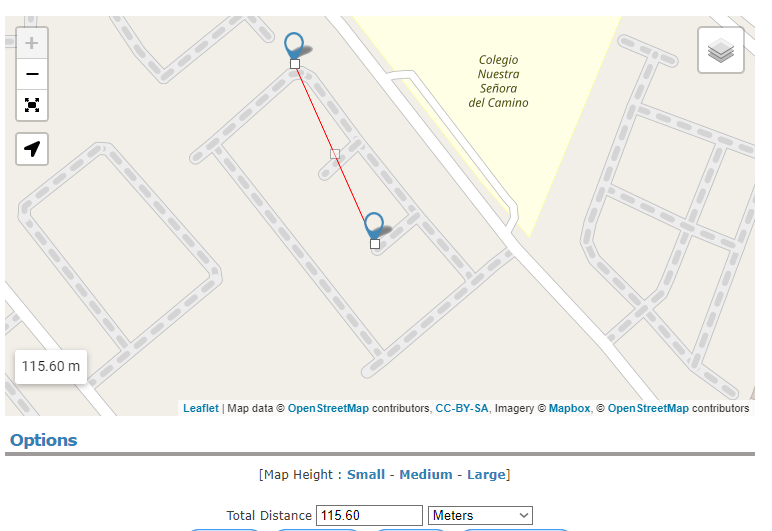
\includegraphics[width = 0.9\textwidth]{imagenes/cap3_resultados/Pruebas LoRa/MapaLora.png}
    \caption{Vista en mapa de distancia máxima de pruebas usando módulo SX1278.}
    \label{fig:mapalora}
\end{figure}

Se modificaron los parámetros del canal y se midió la tasa de paquetes con errores o paquetes corruptos en el receptor. Se realizaron pruebas con los siguientes parámetros fijos:

\begin{itemize}
    \item Frecuencia de operación: 433 MHz.
    \item Tasa de codificación:
    \item Potencia: 10 dBm.
    \item Longitud del preámbulo: 8 bytes.
    \item Tamaño de la carga útil (payload): 128 bytes.
\end{itemize}

Las pruebas se realizaron haciendo uso del módulo Ra-02 de Ai-Thinker, el cual se conectó a un microcontrolador ESP32. En el microcontrolador se implementaron rutinas de envío y recepción de datos medianto rutinas de interrupción (ISR por sus siglas en inglés).

Estos parámetros son recomendados por el fabricante del módulo y se mantuvieron constantes durante las pruebas. Estos se confirmaron tras pruebas preliminares en las cuales se observó que para \textit{payloads} mayores a 128 bytes el porcentaje de paquetes cuyo CRC era erróneo (data corrupta) aumentaba considerablemente, siendo 128 bytes un valor que disminuía esta proporción. Los parámetros que se modificaron fueron el factor de propagación, el ancho de banda y el período de envío entre paquetes. Los resultados de las pruebas se presentan en la tabla \ref{tab:resultadoslora}.

% Please add the following required packages to your document preamble:
% \usepackage{graphicx}
\begin{table}[H]
    \centering
    \caption{Resultados de pruebas realizadas con módulo de comunicaciones Ra-02.}
    \label{tab:resultadoslora}
    \resizebox{\textwidth}{!}{%
    \begin{tabular}{|c|c|c|c|c|}
    \hline
    \textbf{Configuración} & \textbf{F. de Propagación} & \textbf{Ancho de banda} & \textbf{Período} & \textbf{Tasa de paquetes perdidos} \\ \hline
    1 & 9 & 125 kHz & 500 ms & 105/500 \\ \hline
    2 & \textbf{7} & 250 kHz & 150 ms & 1/500 \\ \hline
    3 & \textbf{8} & 125 kHz & 150 ms & 300/500 \\ \hline
    4 & \textbf{8} & 250 kHz & 500 ms & 2/500 \\ \hline
    5 & \textbf{8} & 250 kHz & 200 ms & Error de CRC \\ \hline
    6 & \textbf{7} & 250 kHz & 250 ms & 2/500 \\ \hline
    7 & \textbf{7} & 250 kHz & 200 ms & 2/500 \\ \hline
    8 & \textbf{7} & 250 kHz & 150 ms & 2/500 \\ \hline
    9 & \textbf{7} & 250 kHz & 100 ms & Error de CRC \\ \hline
    \end{tabular}%
    }
\end{table}

Basados en estos resultados, se escogió la configuración 8 para las pruebas de comunicaciones, ya que es la que presenta la menor tasa de paquetes corruptos a la velocidad más alta de envío de paquetes. Esta configuración se utilizó para las pruebas de estimación de inclinación y para las pruebas de funcionamiento del prototipo.

\section{Pruebas para estimación de inclinación}

Para escoger el método de estimación de ángulos, se compararon los siguientes:

\begin{itemize}
    \item Cálculo trigonométrico a partir de mediciones de acelerómetro.
    \item Filtro de Kalman.
    \item Filtro de Madgwick.
\end{itemize}

 Para observar el comportamiento de cada método, se observaron los resultados en un graficador de datos seriales disponible de forma libre, llamado \textit{TelePlot}, creado por Alexander Brehmer. Este funciona como extensión a Visual Studio Code y permite graficar los datos provenientes del puerto serial escogido a una velocidad de transmisión fija. Se realizaron pruebas con cada método y se compararon los resultados obtenidos. 

 \begin{figure}[H]
    \centering
    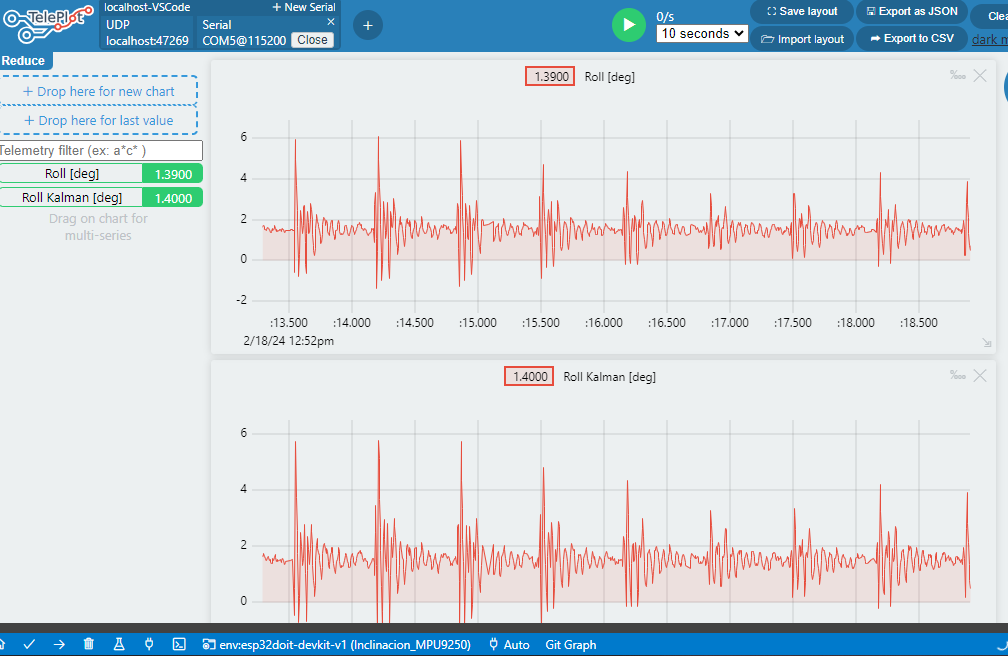
\includegraphics[width = 0.8\textwidth]{imagenes/cap3_resultados/Pruebas ACL/Inclinacion/Comparacion entre Metodo1 (ACL) y Metodo 2 (Kalman) ante vibraciones.png}
    \caption{Entorno TelePlot.}
    \label{fig:teleplot}
\end{figure}

Se realizaron pruebas ante vibración ambiental, ante vibraciones forzadas como golpes y ante movimientos sostenidos para ver el cambio en el ángulo ejecutando los 3 algoritmos al mismo tiempo y haciendo uso del acelerómetro de 9 grados de libertad MPU9250 de Invensense. 

Los resultados gráficos de las pruebas ante vibración ambiental se presentan en la figura \ref{fig:pruebasinclinacion}.

 \begin{figure}[H]
    \centering
    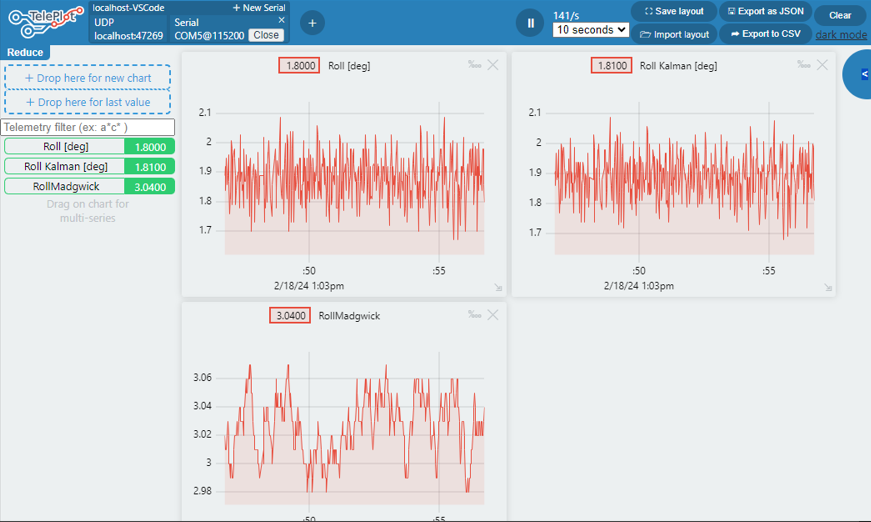
\includegraphics[width = 0.8\textwidth]{imagenes/cap3_resultados/Pruebas ACL/Inclinacion/PruebaInclinacion.png}
    \caption{Comparación entre métodos de estimación de inclinación en vibración ambiental.}
    \label{fig:pruebasinclinacion}
\end{figure}

Al golpear y soplar cerca del sensor, se obtuvieron los siguientes resultados:

\begin{figure}[H]
    \centering
    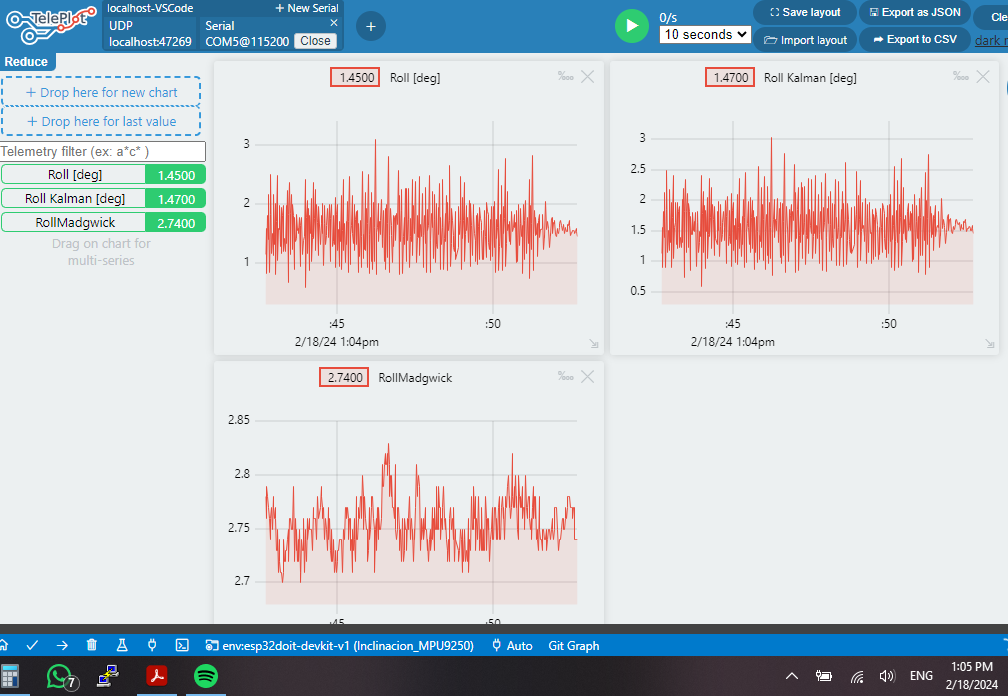
\includegraphics[width = 0.9\textwidth]{imagenes/cap3_resultados/Pruebas ACL/Inclinacion/Comparacion M1 M2 M3 (Maggwick) ante vibraciones.png}
    \caption{Comparación entre métodos de estimación de inclinación ante vibraciones.}
    \label{fig:pruebasinclinacion2}
\end{figure}


Por último, se observó el desempeño de los algoritmos ante movimientos sostenidos que cambiaran el ángulo en el eje de interés:

\begin{figure}[H]
    \centering
    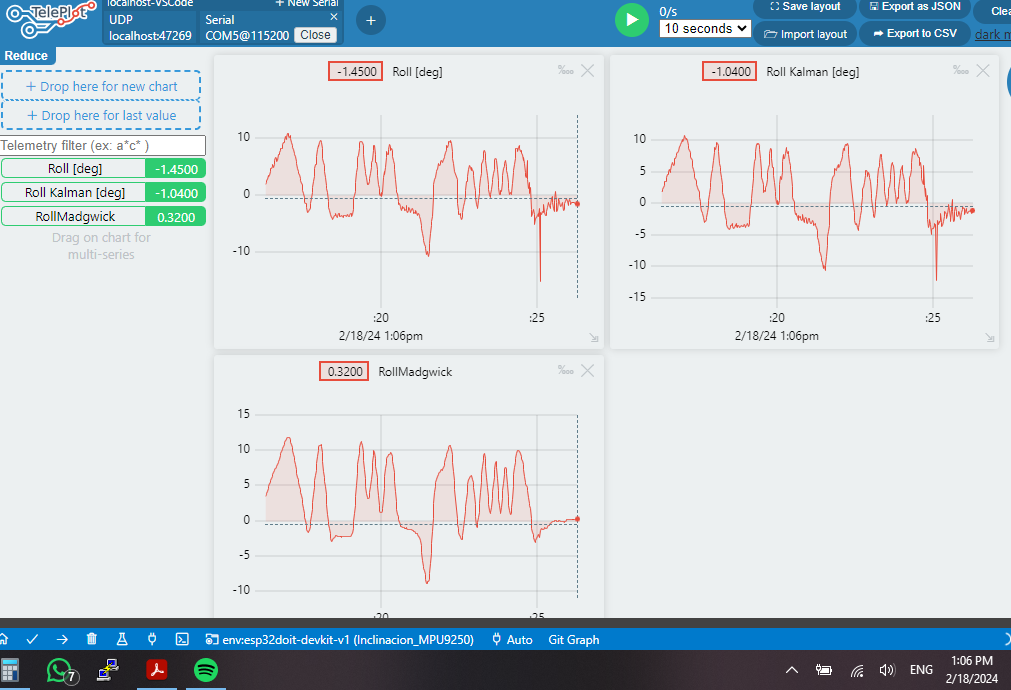
\includegraphics[width = 0.8\textwidth]{imagenes/cap3_resultados/Pruebas ACL/Inclinacion/Comparacion M1 M2 M3 (Maggwick) ante movimiento aleatorios.png}
    \caption{Comparación entre métodos de estimación de inclinación ante movimientos sostenidos.}
    \label{fig:pruebasinclinacion3}
\end{figure}

Se observa claramente en las figuras \ref{fig:pruebasinclinacion}, \ref{fig:pruebasinclinacion2} y \ref{fig:pruebasinclinacion3} que el filtro de Madgwick es el que presenta el mejor desempeño ante vibraciones, golpes y movimientos sostenidos, ya que suaviza las variaciones bruscas en el ángulo. De igual forma, ante vibración ambiental se observa que el filtro de Madgwick es el que presenta un comportamiento más estable, viéndose incluso la resolución en términos de LSB (\textit{Least Significant Bit}) del acelerómetro.

Por lo tanto, se escogió el filtro de Madgwick para la estimación de inclinación en el prototipo.

\section{Pruebas de funcionamiento del prototipo}

Para probar el funcionamiento del prototipo y comparar los resultados obtenidos con un equipo comercial, se llevó a cabo un estudio de vibración sobre una estructura de acero ubicada en el Instituto de Materiales y Modelos Estructurales (IMME) de la Universidad Central de Venezuela. 

La estructura es de tipo aporticada, con una altura de 2,20 metros y una longitud de 2 metros. Cuenta con 4 columnas de acero y distintas vigas con perfil "C" o de canal. El techo de la estructura se encuentra en voladizo, es decir, no está soportado por ninguna columna. La estructura se encuentra en el edificio norte del IMME y se suele utilizar para hacer ensayos de permeabilidad del concreto. Se escogió esta estructura debido a la facilidad para la instrumentación de la misma para realizar las pruebas, siendo esta de poca altura y estando ubicada en un espacio abierto y de fácil acceso por el personal del IMME.

El equipo de medición utilizado para la comparación está basado en la tarjeta de adquisición de datos de \textit{National Instruments} PCI-6221, cuyas características se describen en la tabla \ref{tab:specs6221}, y que puede observarse en la figura  en conjunto con 

%ESPECIFICACIONES DEL DAQ6221

\begin{figure}[H]
    \centering
    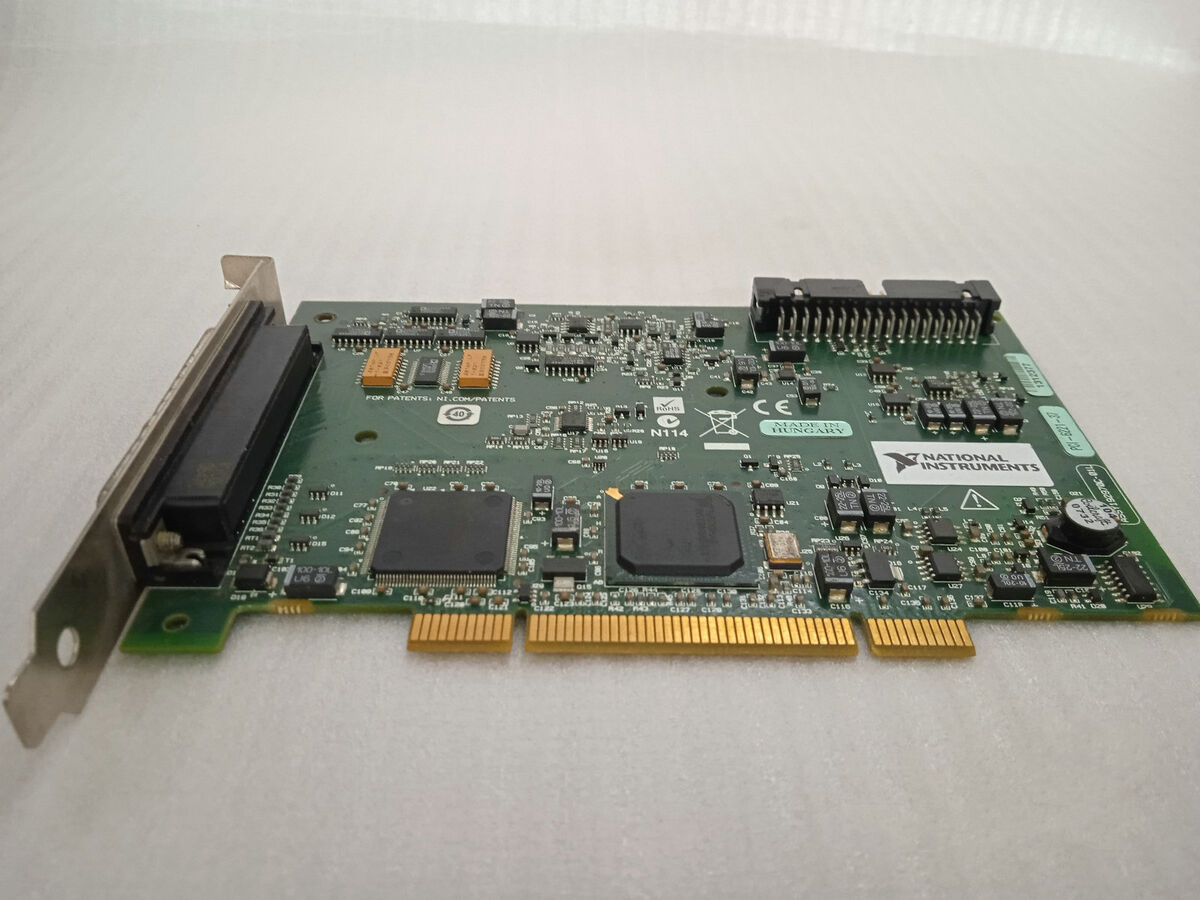
\includegraphics[width = 0.8\textwidth]{imagenes/cap3_resultados/Ensayos/NationalInstruments_PCI6221.jpg}
    \caption{Tarjeta de adquisición de datos PCI-6221 de National Instruments.}
    \label{fig:DAQ6221}
\end{figure}

\begin{figure}[H]
    \centering
    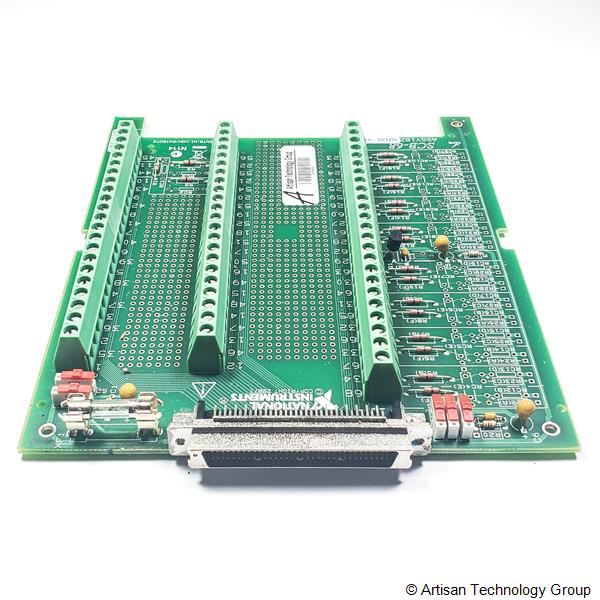
\includegraphics[width = 0.8\textwidth]{imagenes/cap3_resultados/Ensayos/National_Instruments_SCB_68.jpg}
    \caption{Tarjeta de conexiones SCB-68 de National Instruments (Artisan Technology).}
    \label{fig:SCB68}
\end{figure}

% Please add the following required packages to your document preamble:
% \usepackage{graphicx}
\begin{table}[H]
    \centering
    \caption{Especificaciones de la tarjeta de adquisición PCI-6221 de National Instruments}
    \label{tab:specs6221}
    \resizebox{\textwidth}{!}{%
    \begin{tabular}{|c|c|}
    \hline
    \textbf{Parámetro} & \textbf{Valor} \\ \hline
    Número de canales & 8 diferenciales o 16 de un solo canal \\ \hline
    Resolución del ADC & 16 bits \\ \hline
    Tasa de muestreo & 250 kS/s \\ \hline
    Rango de entrada & $\pm 0.2 V, \pm 1 V, \pm 5 V, \pm 10 V$ \\ \hline
    CMRR (Rechazo del modo común) & 92dB \\ \hline
    Tamaño del FIFO de entrada & 4095 muestras \\ \hline
    Exactitud estándar (100 muestras, $\Delta T = 10  C^\circ $) & $3100 \mu V$ \\ \hline
    \end{tabular}%
    }
\end{table}

Los sensores utilizados para el ensayo fueron acelerómetros de balance de fuerza de 1 eje modelo \textit{FBA-11} de la marca \textit{Kinemetrics}. Las características de estos sensores se describen en la tabla \ref{tab:specsFBA11} y puede observarse en la figura \ref{fig:FBA11}. El funcionamiento de este tipo de acelerómetros se describe en detalle en la sección \ref{subsec:sensmonitoreo}.

%ESPECIFICACIONES DEL FBA11

\begin{figure}[H]
    \centering
    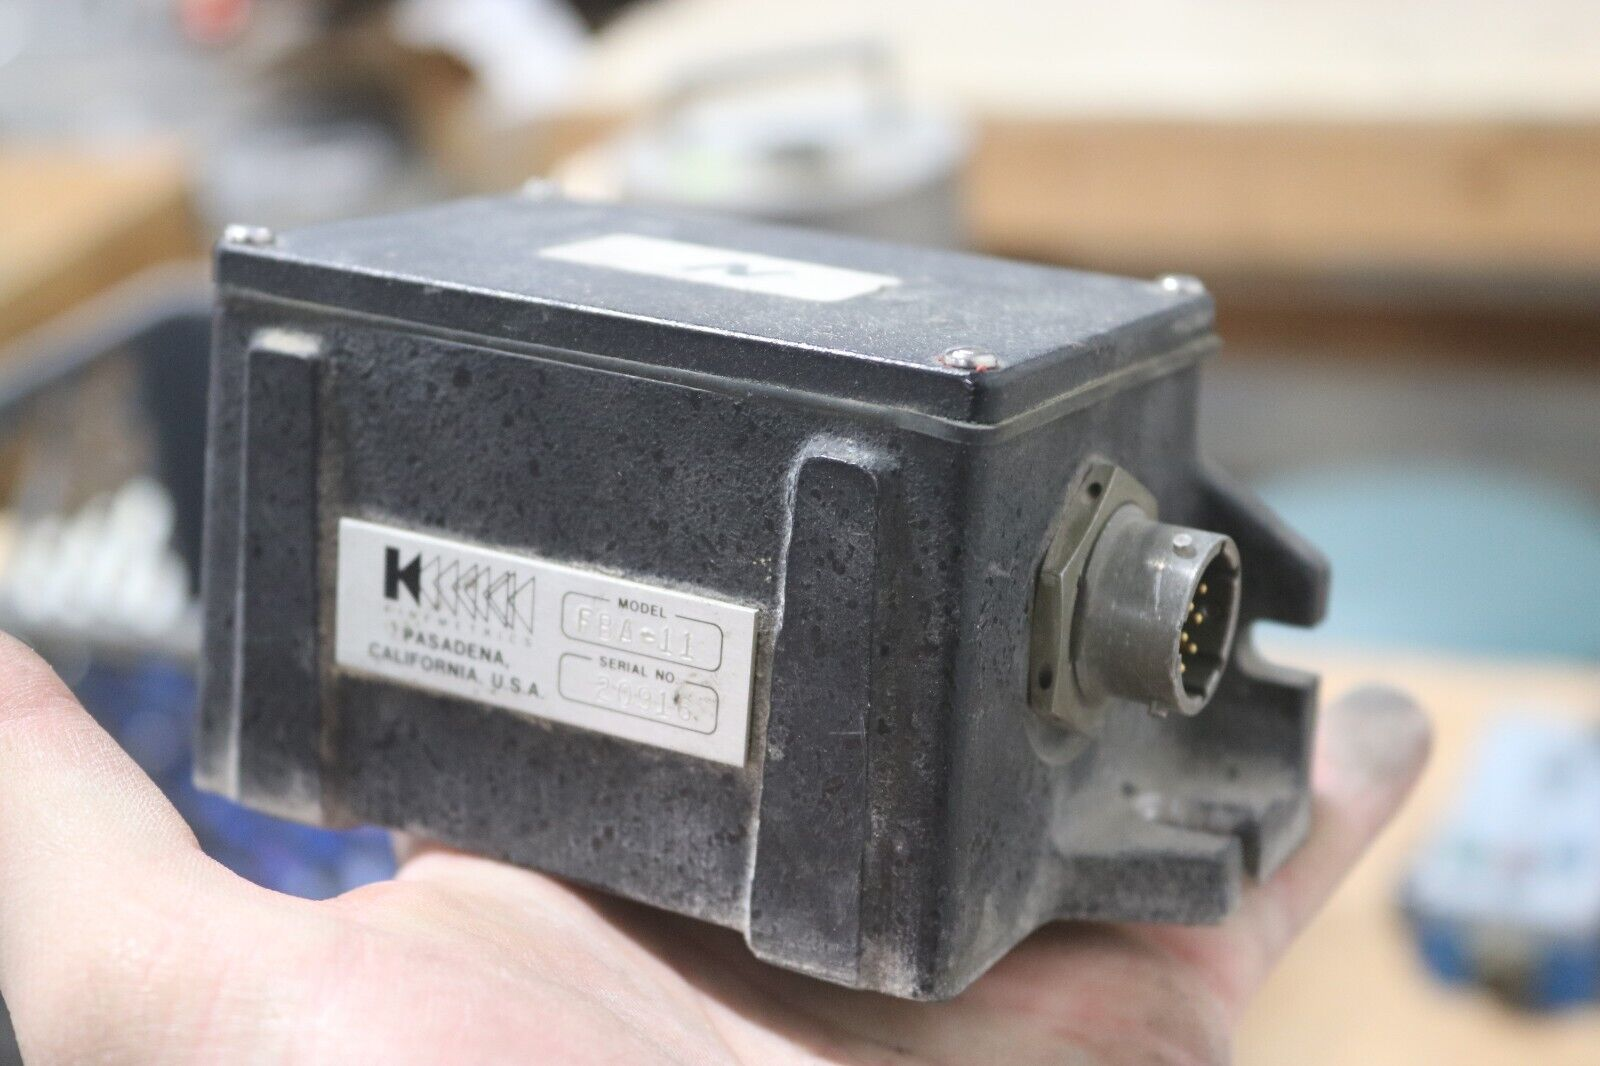
\includegraphics[width = 0.8\textwidth]{imagenes/cap3_resultados/Ensayos/FBA11.jpg}
    \caption{Acelerómetro FBA-11 de Kinemetrics.}
    \label{fig:FBA11}
\end{figure}

% Please add the following required packages to your document preamble:
% \usepackage{graphicx}
\begin{table}[H]
    \centering
    \caption{Especificaciones del acelerómetro FBA-11 de Kinemetrics}
    \label{tab:specsFBA11}
    \resizebox{\textwidth}{!}{%
    \begin{tabular}{|c|c|}
    \hline
    \textbf{Parámetro} & \textbf{Valor} \\ \hline
    Rango de escala completa & $\pm 1.0 g$ (.1, .25, .5 y 2 g opcionales) \\ \hline
    Frecuencia Natural & 50 Hz \\ \hline
    Amortiguamiento & 70\% \\ \hline
    Salida & $\pm 2.5 V / 1 g$ \\ \hline
    Linealidad & Menos de 1\% \\ \hline
    Ruido (entre 0 - 50 Hz) & $\pm 2.5 \mu V$ \\ \hline
    Rango dinámico & 130dB de 0.01 a 50Hz \\ \hline
    Alimentación & $\pm 12 Vdc$ (2.5 mA por eje) \\ \hline
    \end{tabular}%
    }
    \end{table}

Este equipo es el que se utiliza comúnmente en el IMME para realizar ensayos de vibración en estructuras.

El programa para la adquisición de los datos fue diseñado en LabVIEW 8.20 (Versión 2006), el cual es un software de programación gráfica desarrollado por National Instruments. Este programa se encarga de adquirir los datos de los sensores, procesarlos y graficarlos en tiempo real.

Para fijar los sensores se utilizó yeso, como es común en los ensayos de vibración para acoplar los sensores a la estructura.

Los ensayos se dividieron en 3 partes:
\begin{itemize}
    \item Vibración ambiental.
    \item Vibración forzada por impacto.
    \item Vibración libre por condición inicial.
\end{itemize}

La configuración utilizada se puede observar en las figuras \ref{fig:configuracionensayofrontal} y \ref{fig:configuracionensayoplanta} .

\begin{figure}[H]
    \centering
    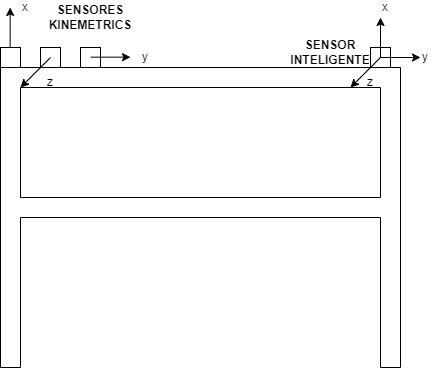
\includegraphics[width = 0.8\textwidth]{imagenes/cap3_resultados/Ensayos/CONFIGURACION1.png}
    \caption{Vista frontal de la configuración utilizada en ensayo.}
    \label{fig:configuracionensayofrontal}
\end{figure}

\begin{figure}[H]
    \centering
    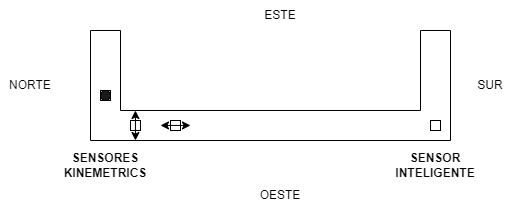
\includegraphics[width = 0.8\textwidth]{imagenes/cap3_resultados/Ensayos/CONFIGURACION1PLANTA.png}
    \caption{Vista de planta de la configuración utilizada en ensayo.}
    \label{fig:configuracionensayoplanta}
\end{figure}


Para comparar los resultados obtenidos con el prototipo y con el equipo comercial, se realizaron las pruebas en paralelo, es decir, se colocaron los sensores del prototipo y del equipo comercial en la estructura y se realizaron las pruebas al mismo tiempo. La instrumentación puede verse en las figuras \ref{fig:inst1} y \ref{fig:inst2}. Los resultados obtenidos se compararon en términos de la respuesta en frecuencia y la respuesta en el tiempo.


\begin{figure}[H]
    \centering
    \subfloat[Vista de la estructura instrumentada con los acelerómetros FBA-11 de Kinemetrics]{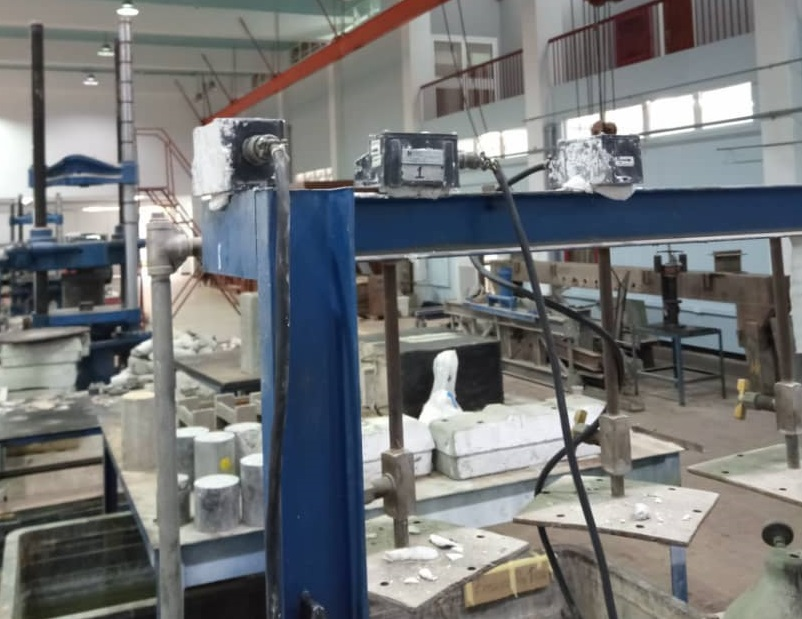
\includegraphics[width = 0.6\textwidth]{imagenes/cap3_resultados/Ensayos/InstrumentacionConf1FBA.jpg}\label{fig:inst1}}
    \hfill
    \subfloat[Vista de la estructura instrumentada incluyendo el prototipo de pruebas]{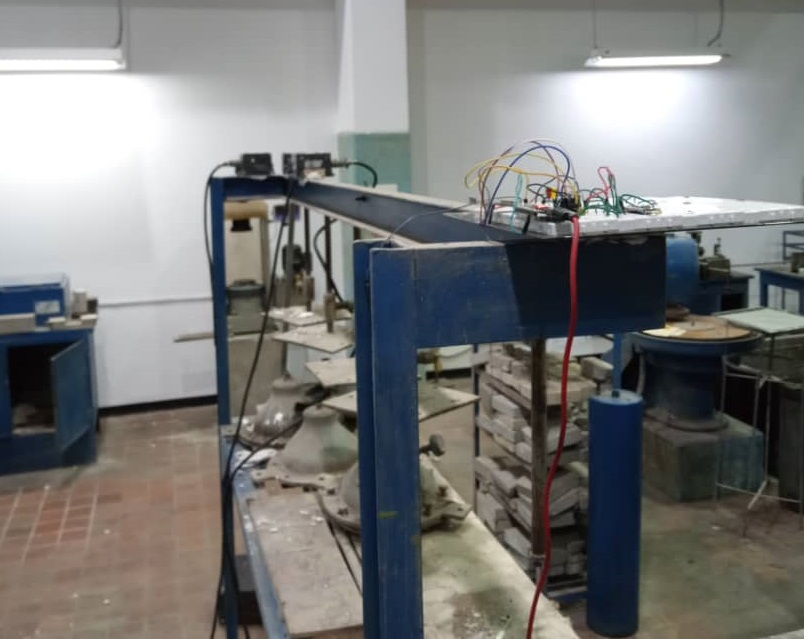
\includegraphics[width = 0.6\textwidth]{imagenes/cap3_resultados/Ensayos/InstrumentacionConf1FBASmartSensor.jpg}\label{fig:inst2}}
    \caption{Instrumentación de la estructura}
    \label{fig:inst}
\end{figure}

Durante el ensayo, el sensor inteligente estaba siendo controlado y monitoreado desde la estación base ubicada a pocos metros de la estructura. En esta estación base se encontraba el computador que , a través de una interfaz gráfica, permitía visualizar los datos en y guardarlos en un archivo de texto para su posterior análisis. El diseño de la interfaz gráfica de usuario puede observarse en las figuras \ref{fig:interfaz1} y \ref{fig:interfaz2}. La programación y características principales de esta interfaz fueron descritas en la sección \ref{subsec:softwaredesc}.

\begin{figure}[H]
    \centering
    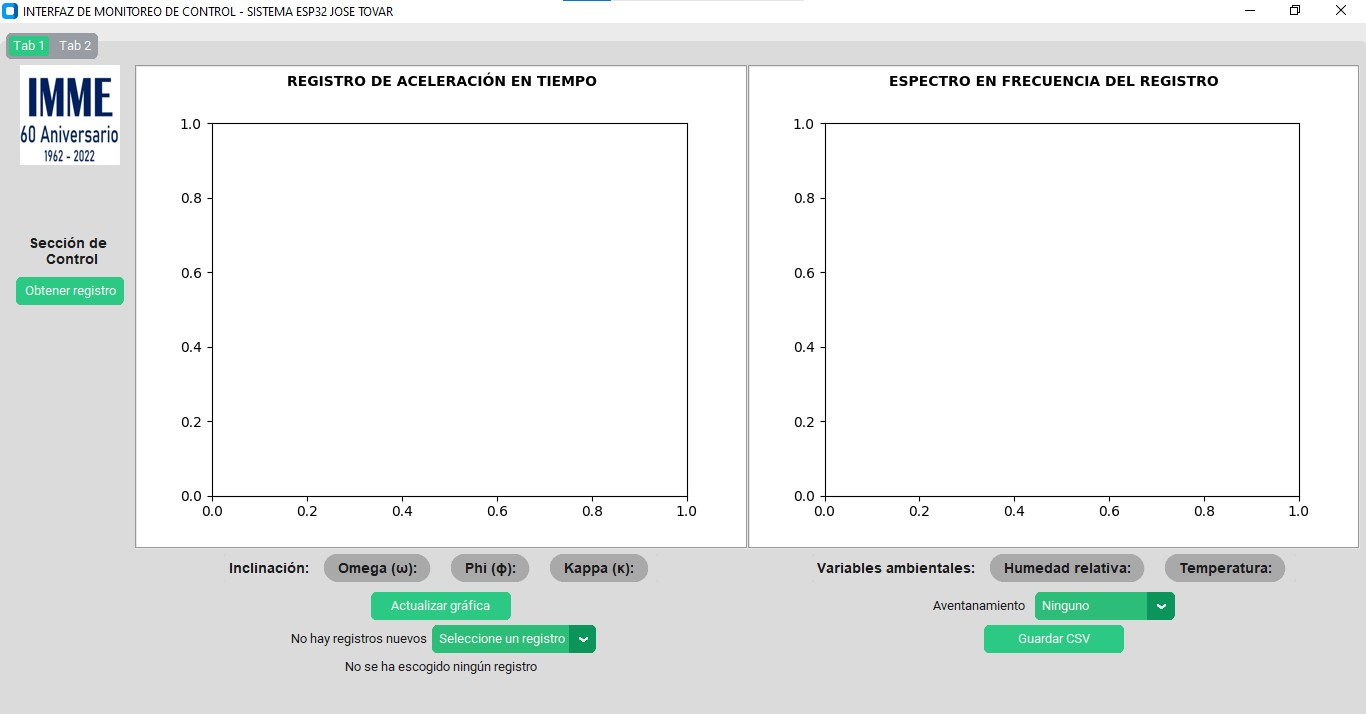
\includegraphics[width = \textwidth]{imagenes/cap3_resultados/Ensayos/GUI1.jpg}
    \caption{Ventana 1 de la interfaz gráfica diseñada.}
    \label{fig:interfaz1}
\end{figure}

\begin{figure}[H]
    \centering
    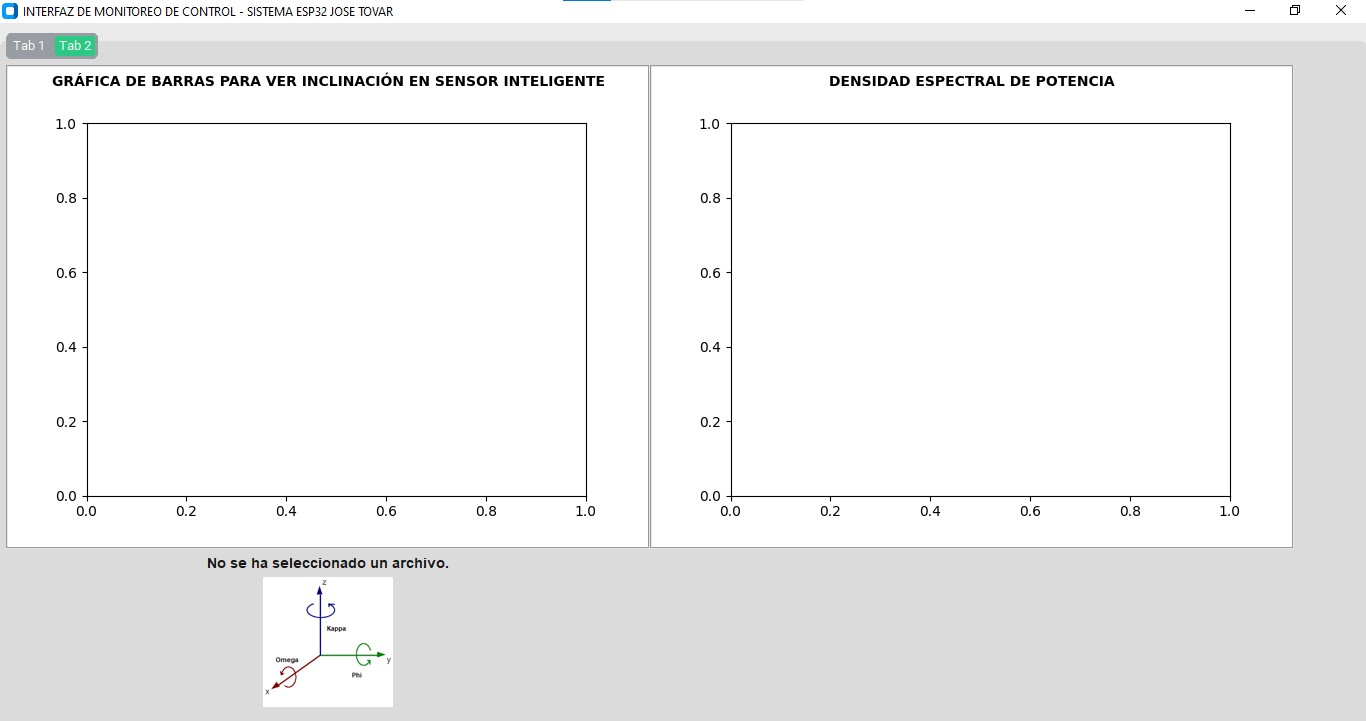
\includegraphics[width = \textwidth]{imagenes/cap3_resultados/Ensayos/GUI2.jpg}
    \caption{Ventana 2 de la interfaz gráfica diseñada.}
    \label{fig:interfaz2}
\end{figure}

Para el procesamiento de los datos obtenidos haciendo uso de la tarjeta de adquisición de datos PCI-6221 se implementó un código en MATLAB, donde, de forma similar a la interfaz de la figura \ref{fig:interfaz1}, se grafican los datos en tiempo real y el espectro en frecuencia correspondiente.

Los datos se importaron directamente del archivo \textit{.lvm} generado por LabView y fueron preprocesados con la interfaz de MATLAB para importar datos de archivos externos, como se puede observar en la figura \ref{fig:datosmatlab}.

\begin{figure}[H]
    \centering
    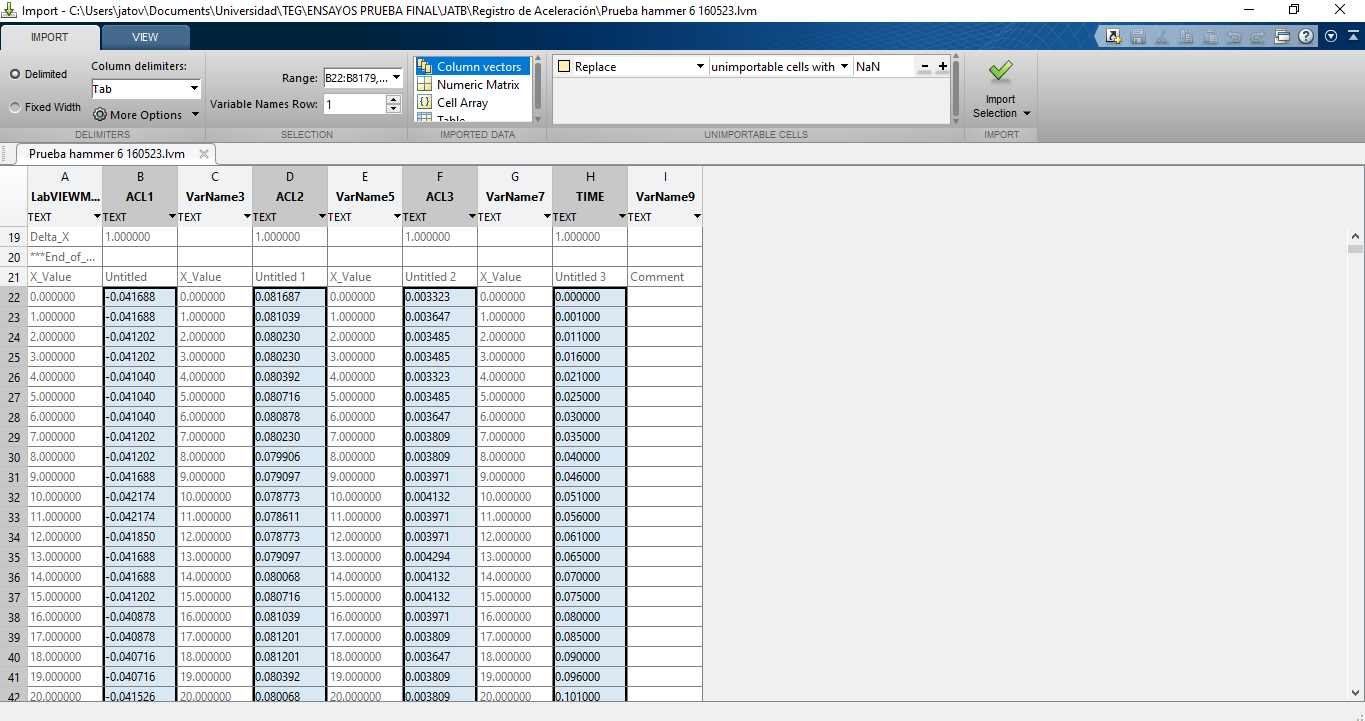
\includegraphics[width = \textwidth]{imagenes/cap3_resultados/Ensayos/datosmatlab.png}
    \caption{Ventana de la interfaz gráfica de MATLAB para importar los datos obtenidos mediante LabVIEW.}
    \label{fig:datosmatlab}
\end{figure}

Las características de instrumentación para ambos sistemas fueron las mostradas en la tabla \ref{tab:comparacionsist}:
% Please add the following required packages to your document preamble:
% \usepackage{graphicx}
\begin{table}[H]
    \centering
    \caption{Comparación entre características de los sistemas de medición utilizados.}
    \label{tab:comparacionsist}
    \resizebox{\textwidth}{!}{%
    \begin{tabular}{|c|c|c|}
    \hline
    \textbf{Parámetro} & \textbf{Sistema basado en PCI6221} & \multicolumn{1}{l|}{\textbf{Sensor inteligente}} \\ \hline
    Frecuencia de muestreo & 200 Hz & 200 Hz \\ \hline
    Número de muestras máx. & 12000 & 1024 \\ \hline
    Alimentación & 120 Vac & 5 Vdc \\ \hline
    Peso aproximado & 25-30 kg & 800 g \\ \hline
    \begin{tabular}[c]{@{}c@{}}Dimensiones aproximadas\\ \end{tabular} & 1,5 m (solo estación base) & 25 cm \\ \hline
    Cableado & Sí & No \\ \hline
    Alerta ante eventos & No & Sí \\ \hline
    \end{tabular}%
    }
    \end{table}

A continuación se presentan y comparan los resultados obtenidos en cada ensayo:

\subsection{Vibración forzada por impacto}

Este ensayo consistió en excitar la estructura haciendo uso de un martillo de goma, haciendo que la misma comience a vibrar. Para este ensayo se contó con la ayuda de personal del IMME para coordinar la toma de datos con el impacto sobre el sistema. Además de buscar la semejanza entre ambos resultados, se buscaba comprobar el efecto que produce un cambio en la masa sobre la frecuencia natural del sistema. Para esto, se añadieron 5 lastres de 17 kg al sistema luego del primer ensayo de vibración por impacto.

En primer lugar, se observa en las figuras \ref{fig:DAQHammer} la respuesta en tiempo y en frecuencia usando el sistema basado en la tarjeta PCI-6221:

\begin{figure}[H]
    \centering
    \subfloat[Aceleración en el tiempo del sistema ante vibración por impacto en dirección Este-Oeste]{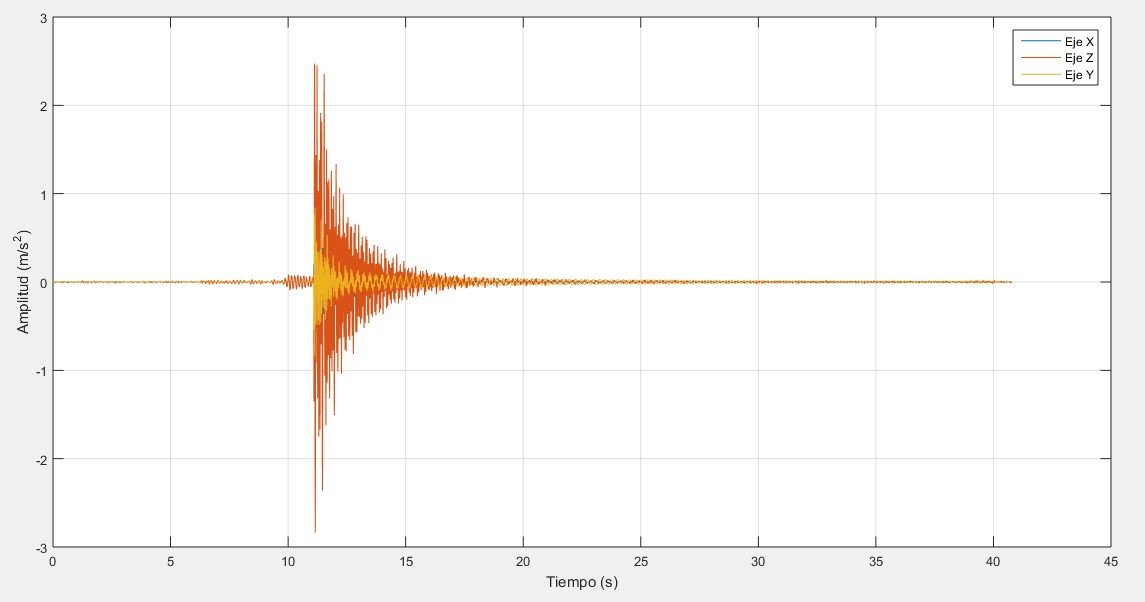
\includegraphics[width = \textwidth]{imagenes/cap3_resultados/Ensayos/VibHammer6EsteOesteNIDAQ.jpg}\label{fig:DAQham1}}
    \hfill
    \subfloat[Espectro en frecuencia del sistema ante vibración por impacto en dirección Este-Oeste]{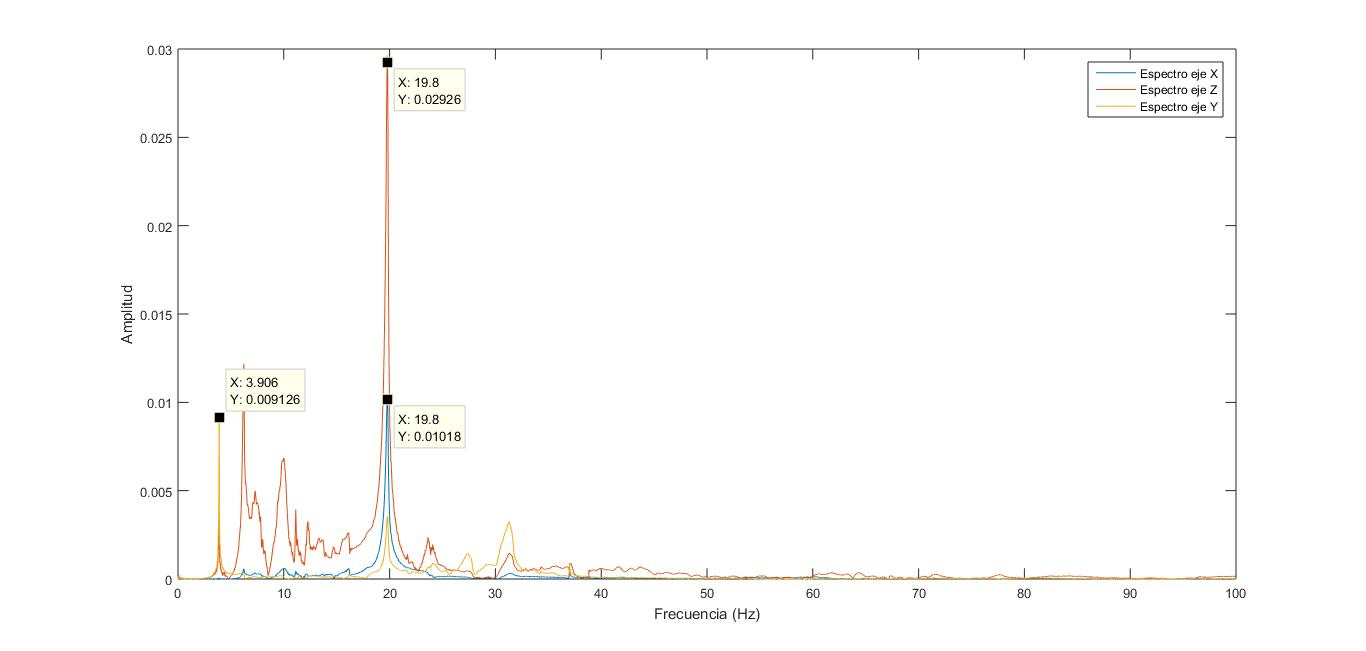
\includegraphics[width = \textwidth]{imagenes/cap3_resultados/Ensayos/VibHammer6EsteOesteEspectroNIDAQ.jpg}\label{fig:DAQham2}}
    \caption{Respuesta del sistema ante vibración por impacto según la tarjeta PCI-6221 de National Instruments}
    \label{fig:DAQHammer}
\end{figure}

El registro obtenido para este mismo impacto haciendo uso del sensor inteligente se puede observar en la figura \ref{fig:impactoGUI}. En la figura \ref{fig:ventana2} se incluye la ventana auxiliar de la interfaz gráfica que permite al operador verificar la inclinación del sensor y si este se encuentra a nivel, así como identificar el ángulo en desnivel para su corrección. También se incluye la gráfica de la densidad espectral de potencia, que en ocasiones permite caracterizar de forma más rápida las frecuencias de vibración, sobre todo en espectros que contienen múltiples frecuencias. La densidad espectral de potencia también es útil para aplicar el método del ancho de banda local, utilizado para estimar el amortiguamiento del sistema.

\begin{figure}[H]
    \centering
    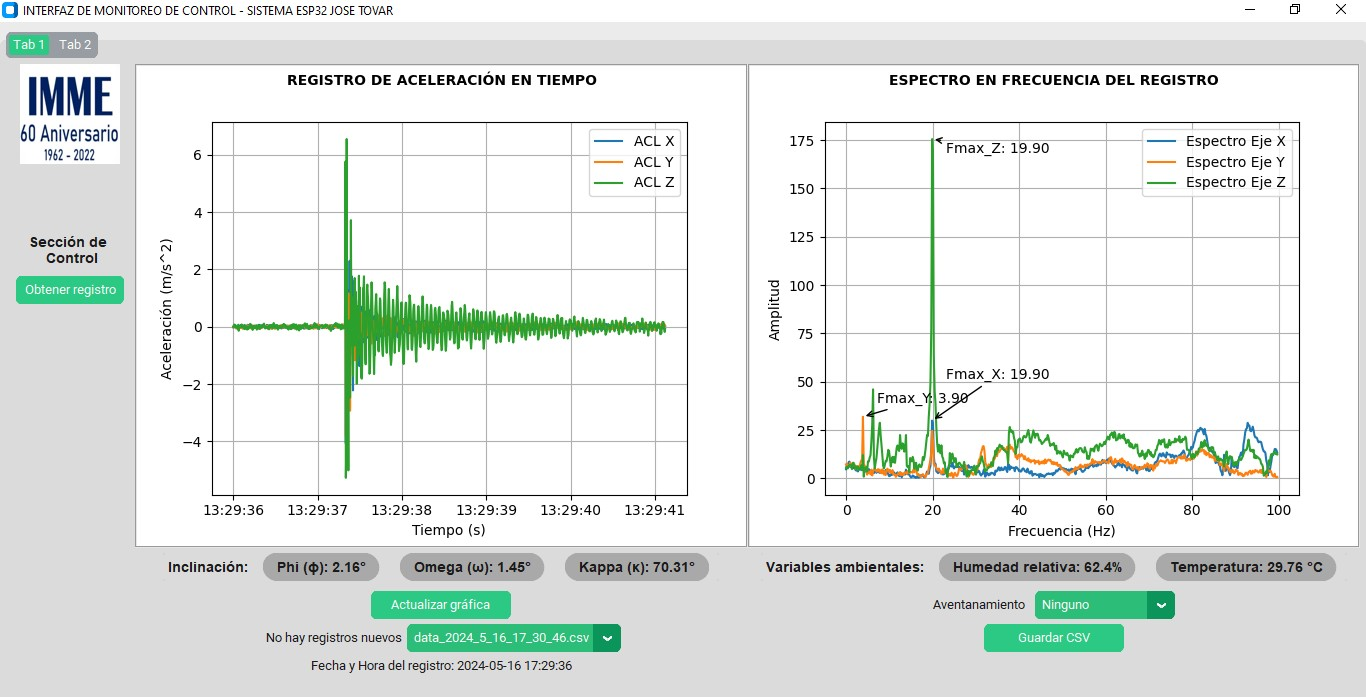
\includegraphics[width = \textwidth]{imagenes/cap3_resultados/Ensayos/VibHammer6EsteOesteSMARTSENSOR.jpg}
    \caption{Registro de vibración por impacto en la dirección Este-Oeste obtenido mediante el sensor inteligente.}
    \label{fig:impactoGUI}
\end{figure}

\begin{figure}[H]
    \centering
    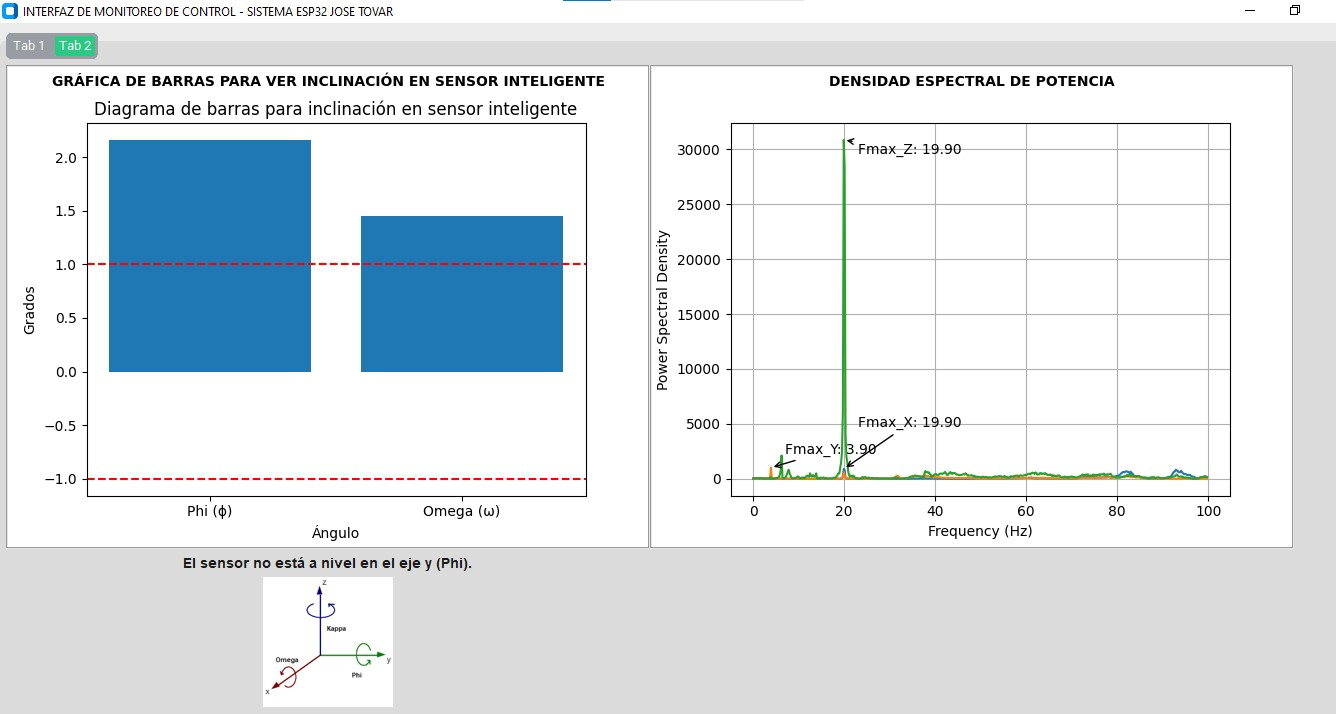
\includegraphics[width = \textwidth]{imagenes/cap3_resultados/Ensayos/VibHammer1NorteSurSMARTSENSORVentana2.jpg}
    \caption{Ventana auxiliar de la GUI para observar la inclinación y la densidad espectral de potencia.}
    \label{fig:ventana2}
\end{figure}

Al comparar los espectros en frecuencia obtenidos en las figuras \ref{fig:DAQham2} y \ref{fig:impactoGUI} se observa que las frecuencias de vibración obtenidas se corresponden entre ambos sistemas de medición, siendo el error entre ambos picos en frecuencia de 0.1 Hz.

Por otro lado, se impactó el sistema sin los lastres en la dirección Norte-Sur, obteniéndose la respuesta observada en la figura \ref{fig:DAQHammerNS} según el sistema basado en la tarjeta PCI-6221:

\begin{figure}[H]
    \centering
    \subfloat[Aceleración en el tiempo del sistema ante vibración por impacto en dirección Norte-Sur]{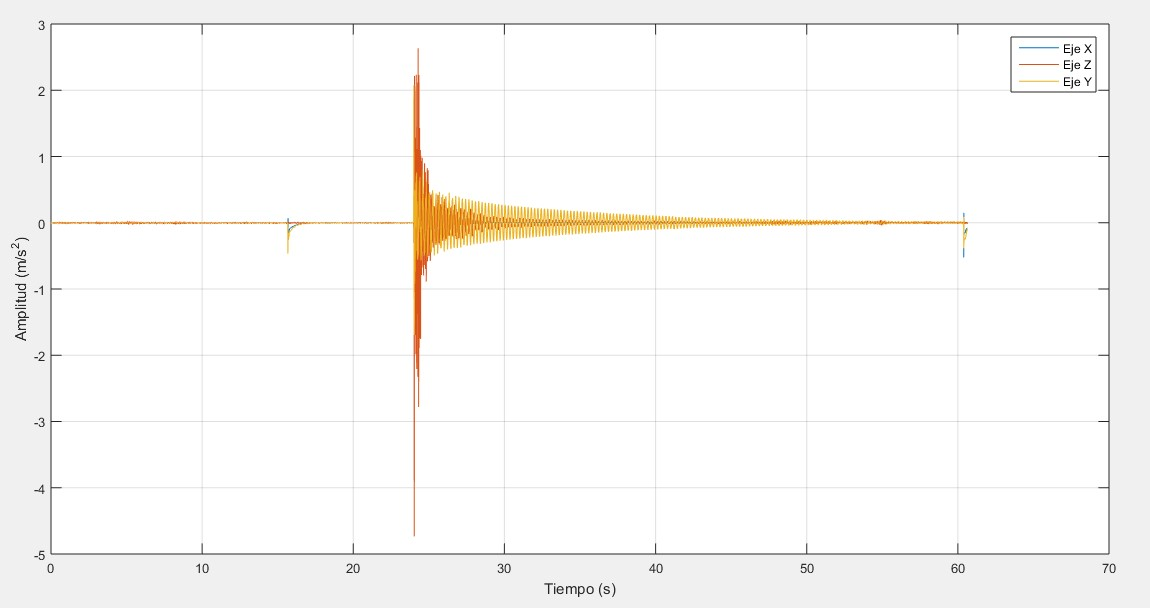
\includegraphics[width = \textwidth]{imagenes/cap3_resultados/Ensayos/VibHammer1NorteSurNIDAQ.jpg}\label{fig:DAQham1NS}}
    \hfill
    \subfloat[Espectro en frecuencia del sistema ante vibración por impacto en dirección Norte-Sur]{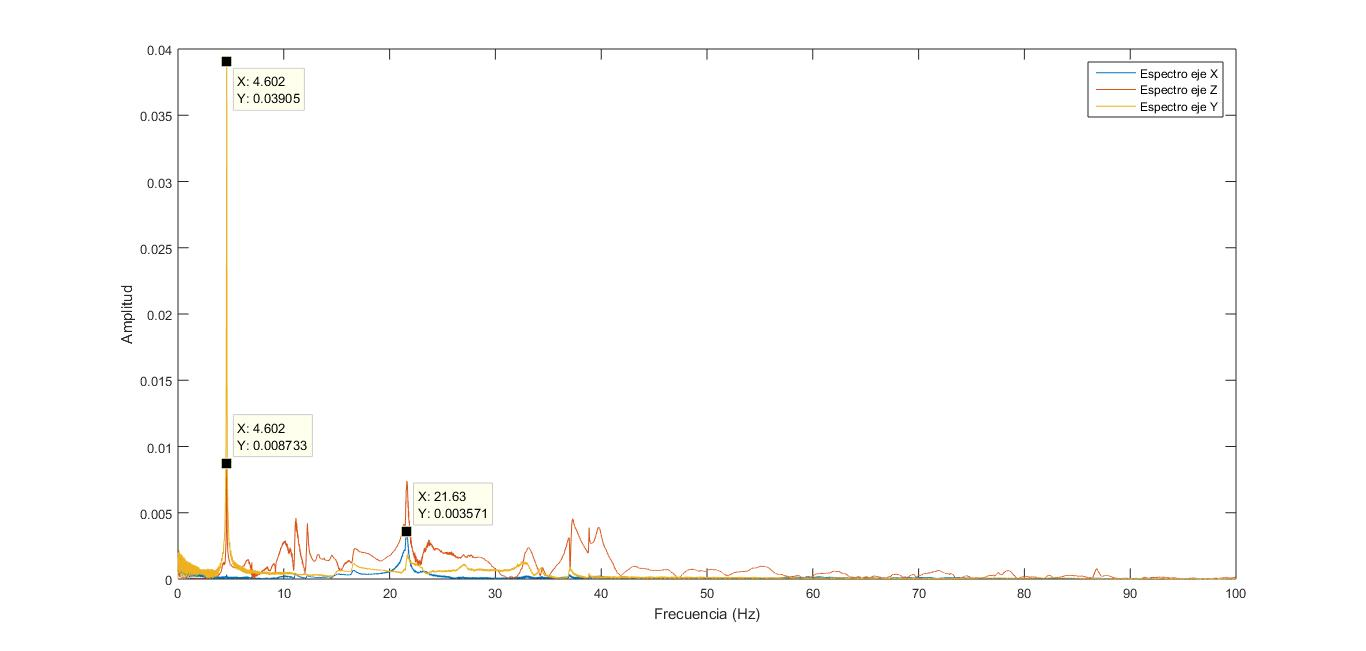
\includegraphics[width = \textwidth]{imagenes/cap3_resultados/Ensayos/VibHammer1NorteSurEspectroNIDAQ.jpg}\label{fig:DAQham2NS}}
    \caption{Respuesta del sistema ante vibración por impacto según la tarjeta PCI-6221 de National Instruments}
    \label{fig:DAQHammerNS}
\end{figure}

Por su parte, el sensor inteligente obtuvo la respuesta del sistema observada en la figura y \ref{fig:impactoGUI_NS}:

\begin{figure}[H]
    \centering
    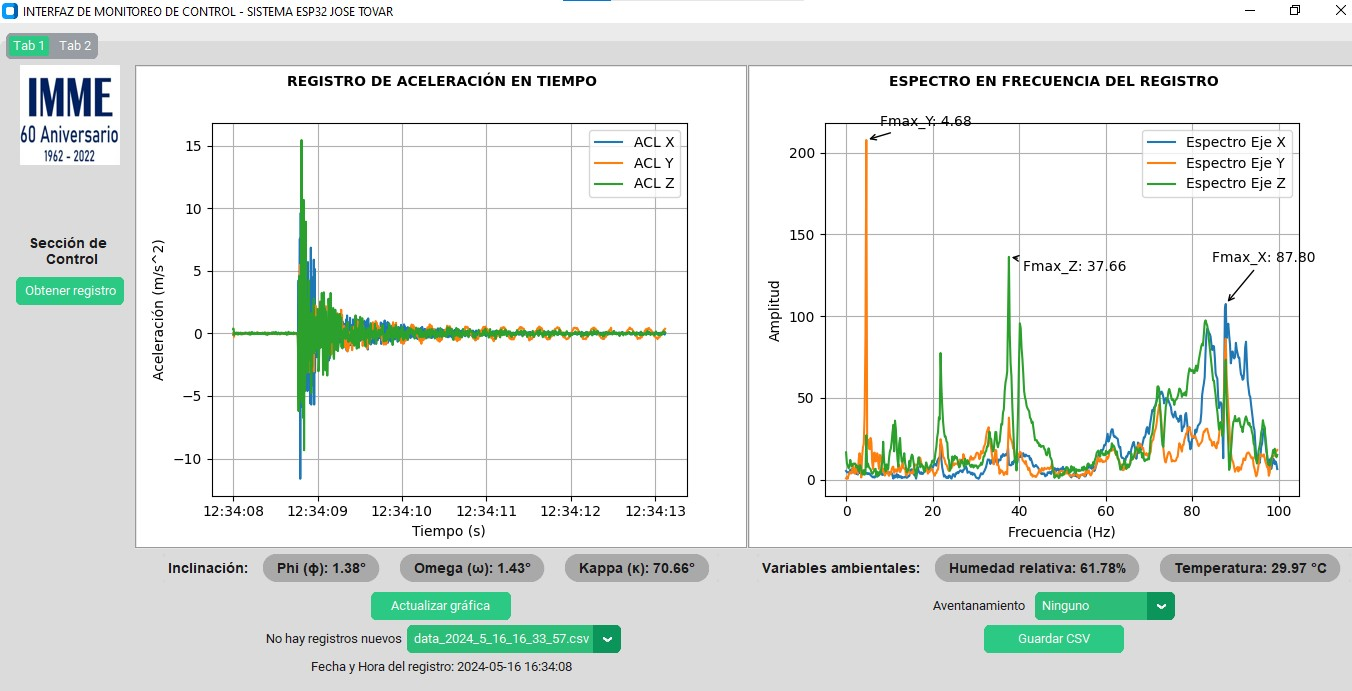
\includegraphics[width = \textwidth]{imagenes/cap3_resultados/Ensayos/VibHammer1NorteSurSMARTSENSOR.jpg}
    \caption{Registro de vibración por impacto en la dirección Norte-Sur obtenido mediante el sensor inteligente.}
    \label{fig:impactoGUI_NS}
\end{figure}

En primer lugar, se observa la gran similitud entre ambas respuestas, siendo la frecuencia de vibración en la dirección larga de 4.6 Hz en ambos sistemas, con un error de 0.08Hz en este caso. Además, se comprueba que el peso influye en la respuesta en frecuencia, al observarse que la frecuencia de vibración en la dirección larga (que en este caso corresponde al eje y por la configuración de los acelerómetros), disminuye al agregarse los lastres, siendo de 4.6 Hz inicialmente, y cambiando a 3.9 Hz luego de agregar los lastres.

\subsection{Vibración libre por condición inicial}

El ensayo de vibración libre consiste en aplicar una condición inicial a la estructura para posteriormente eliminar esta condición, que puede ser un peso o fuerza aplicada, y permitir que la estructura vibre libremente hasta alcanzar su condición de reposo o de vibración ambiental.

En este caso, se realizaron pruebas aplicando una condición inicial en el sentido norte-sur a la estructura y luego se dejó vibrar libremente al retirar la condición inicial. Análogo al ensayo anterior, se hizo el estudio con y sin lastres para evaluar el efecto del cambio en la respuesta dinámica del sistema al variar la masa del sistema.

En las figuras \ref{fig:DAQlibre1SL} y \ref{fig:DAQlibre1SL} se observa la respuesta del sistema en vibración libre antes de la colocación de los 5 lastres de 17 kg:

\begin{figure}[H]
    \centering
    \subfloat[Aceleración en el tiempo del sistema ante vibración libre sin lastres]{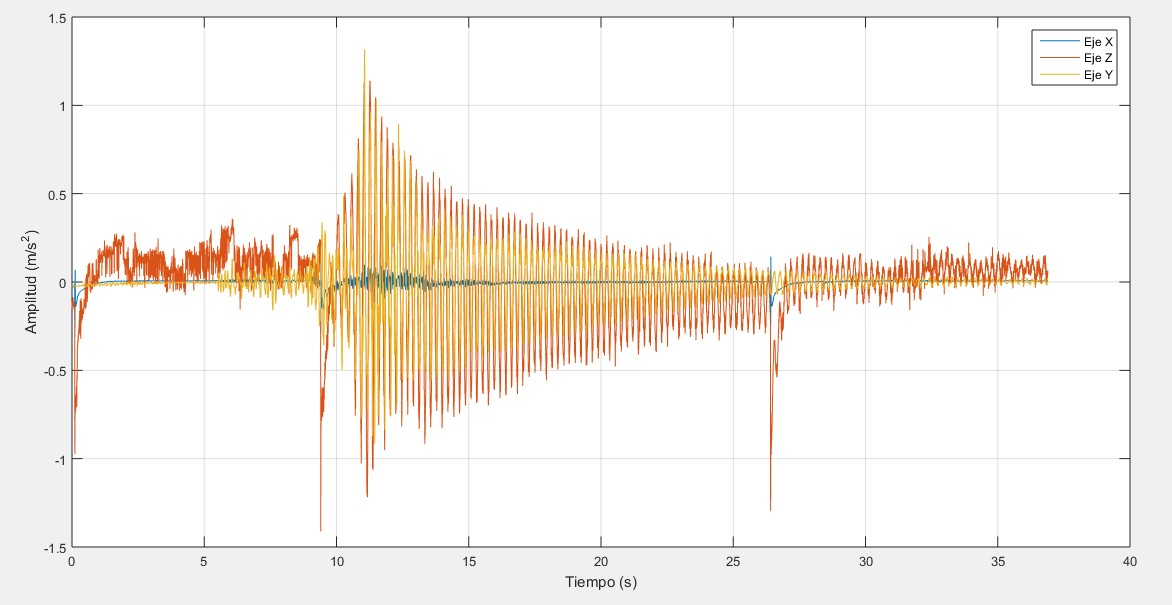
\includegraphics[width = \textwidth]{imagenes/cap3_resultados/Ensayos/AmpVibLibreSinLastresNIDAQ.jpg}\label{fig:DAQlibre1SL}}
    \hfill
    \subfloat[Espectro en frecuencia del sistema ante vibración libre sin lastres]{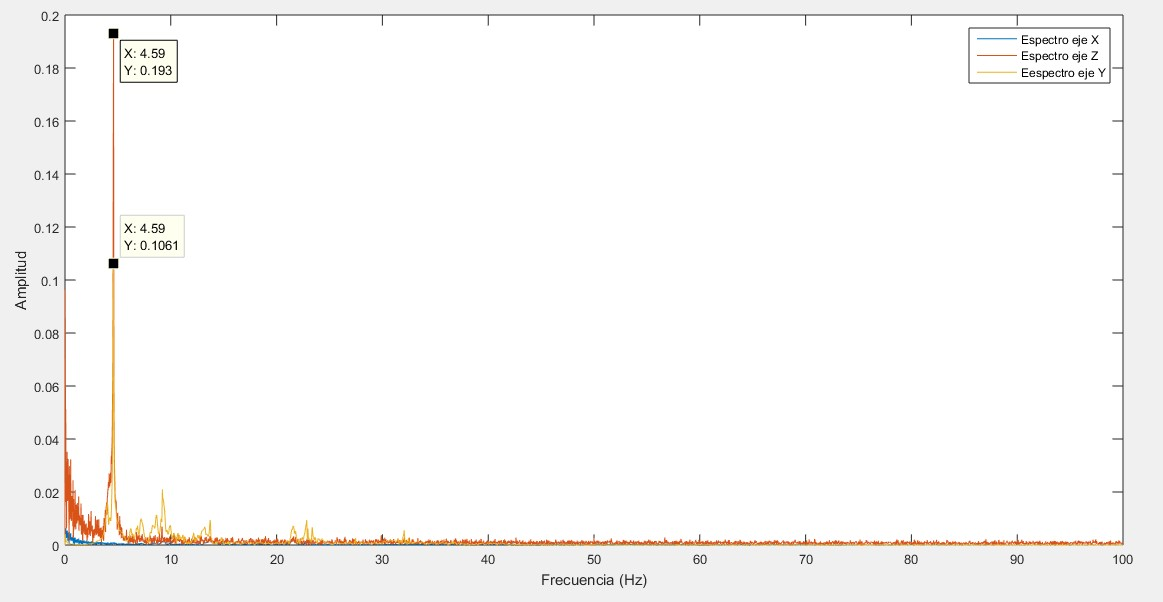
\includegraphics[width = \textwidth]{imagenes/cap3_resultados/Ensayos/VibLibreSinLastresNIDAQ.jpg}\label{fig:DAQlibre2SL}}
    \caption{Respuesta del sistema ante vibración libre sin lastres según la tarjeta PCI-6221 de National Instruments}
    \label{fig:DAQlibreSL}
\end{figure}

Por su parte, la respuesta obtenida por el sensor inteligente durante este ensayo se observa en la figura 

\begin{figure}[H]
    \centering
    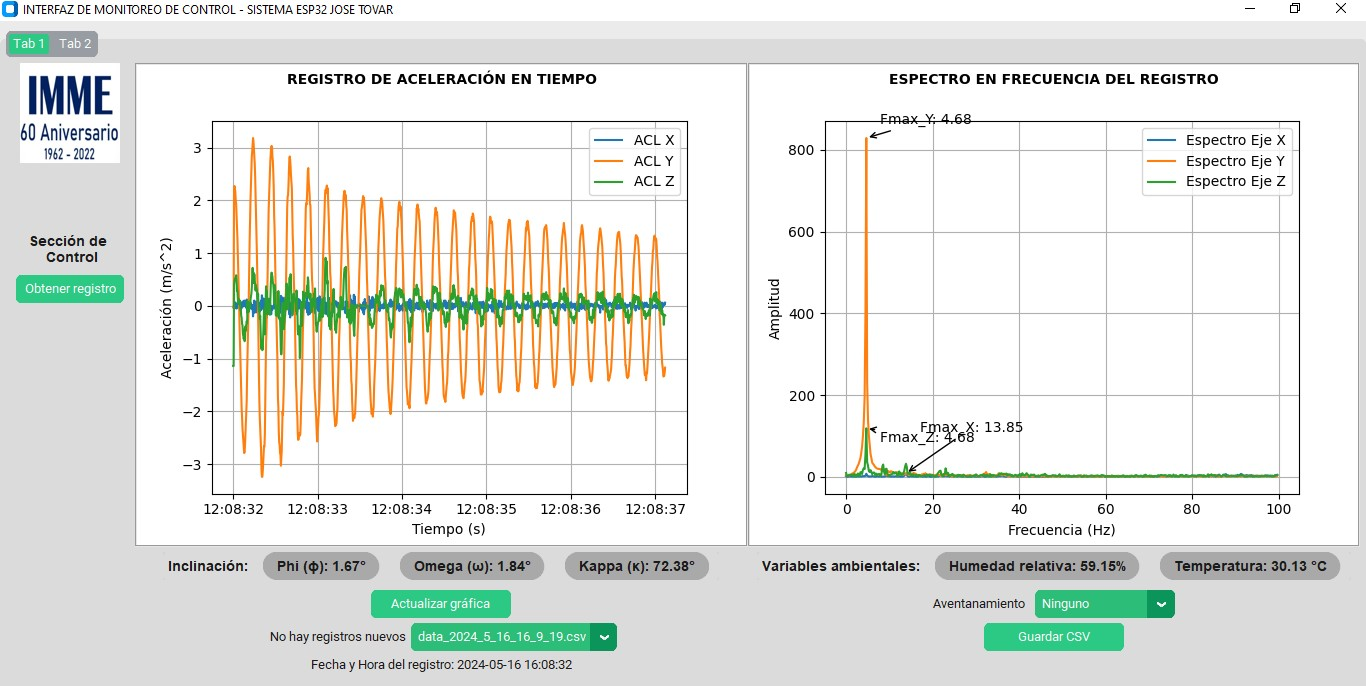
\includegraphics[width = \textwidth]{imagenes/cap3_resultados/Ensayos/VibLibreSinLastresSMARTSENSOR.jpg}
    \caption{Registro de vibración libre sin lastres obtenido mediante el sensor inteligente.}
    \label{fig:libreGUI_SL}
\end{figure}

Al comparar los resultados obtenidos en el espectro en frecuencia usando ambos sistemas, como se ve en las figuras \ref{fig:libreGUI_SL} y \ref{fig:DAQlibreSL}, se observa la similitud entre el espectro en frecuencia del sistema basado en el sensor inteligente diseñado y el sistema comercial disponible en el IMME. En este caso, la diferencia entre la frecuencia natural del sistema en la dirección Norte-Sur obtenida por el sensor inteligente en comparación a la obtenida por la tarjeta PCI-6221 es de 0.09Hz, observándose además que el sensor inteligente mostró un comportamiento estable mientras que el sistema basado en la tarjeta de adquisición presenta problemas de deriva y picos indeseados que agregan componentes frecuenciales ajenas al sistema estructural, demostrándose así la confiabilidad del sensor inteligente.


De igual forma, se ejecutó la misma prueba luego de añadir los lastres, obteniéndose los resultados mostrados en la figura \ref{fig:DAQlibreCL}:
\begin{figure}[H]
    \centering
    \subfloat[Aceleración en el tiempo del sistema ante vibración libre con lastres]{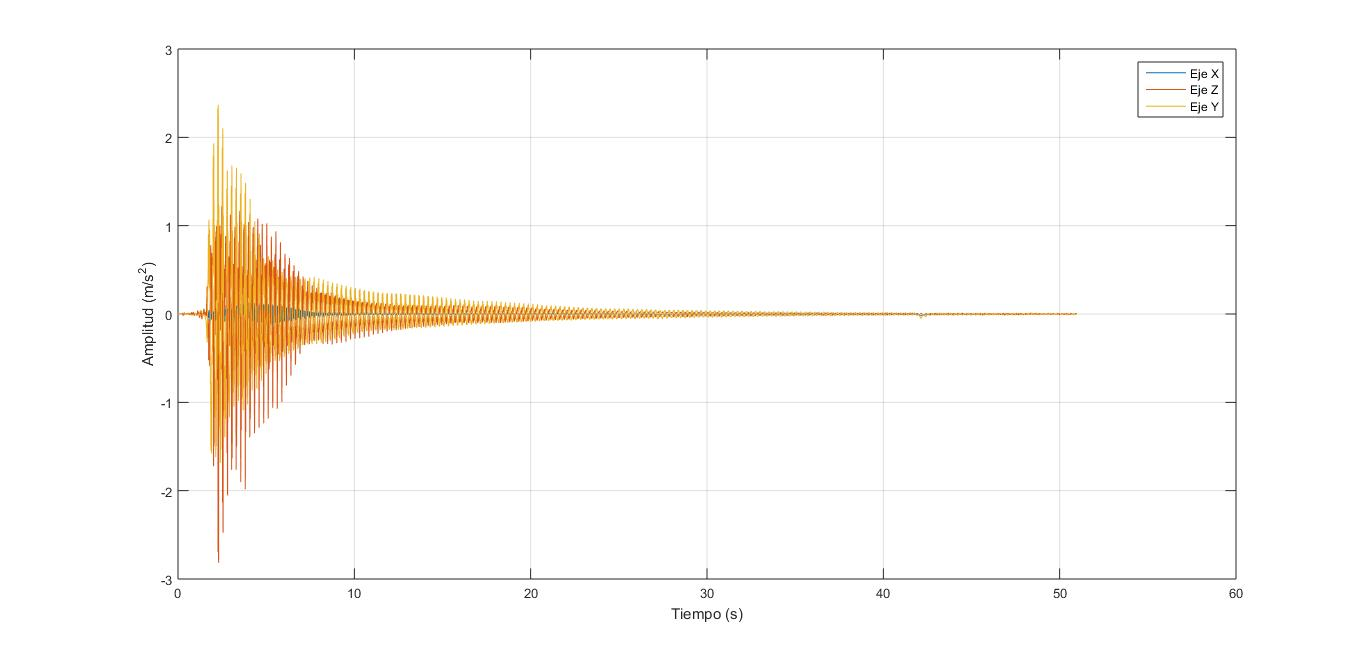
\includegraphics[width = \textwidth]{imagenes/cap3_resultados/Ensayos/AmplitudVibLibreLastresNIDAQ1.jpg}\label{fig:DAQlibre1CL}}
    \hfill
    \subfloat[Espectro en frecuencia del sistema ante vibración libre con lastres]{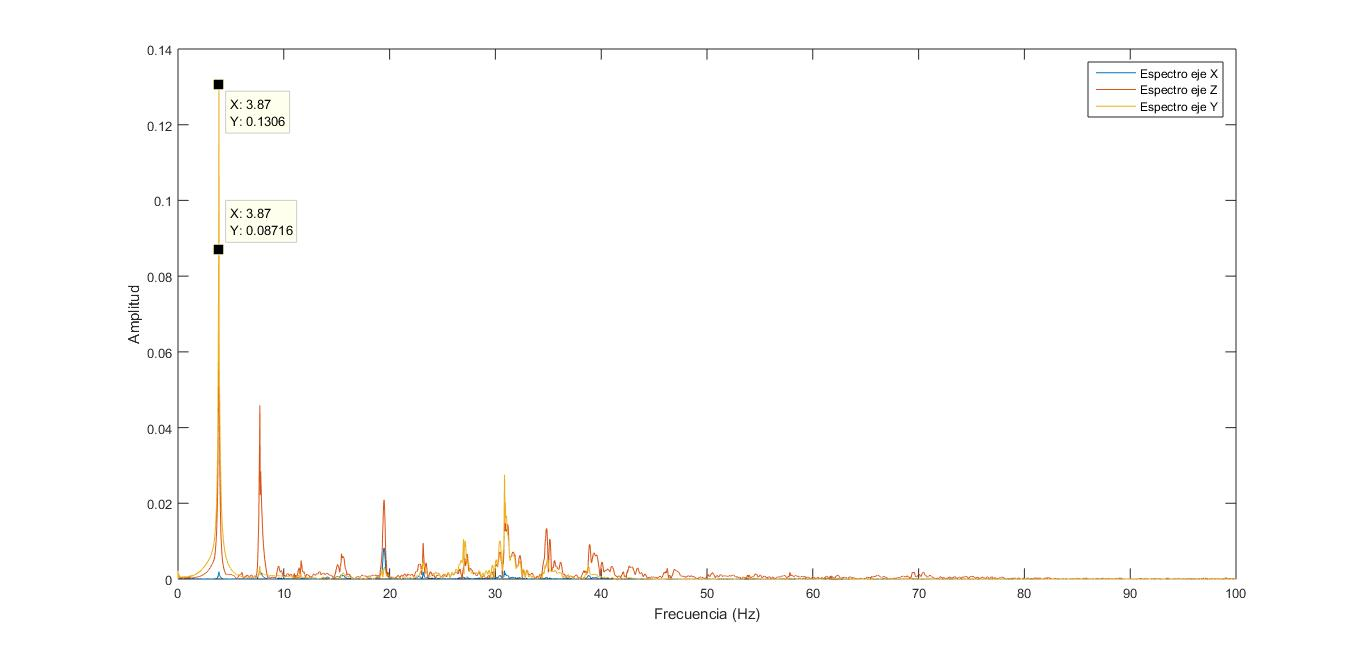
\includegraphics[width = \textwidth]{imagenes/cap3_resultados/Ensayos/VibLibreLastresNIDAQ1.jpg}\label{fig:DAQlibre2CL}}
    \caption{Respuesta del sistema ante vibración libre con lastres según la tarjeta PCI-6221 de National Instruments}
    \label{fig:DAQlibreCL}
\end{figure}


Mientras que en la figura \ref{fig:libreGUI_CL} se observan los resultados arrojados por el sensor inteligente:

\begin{figure}[H]
    \centering
    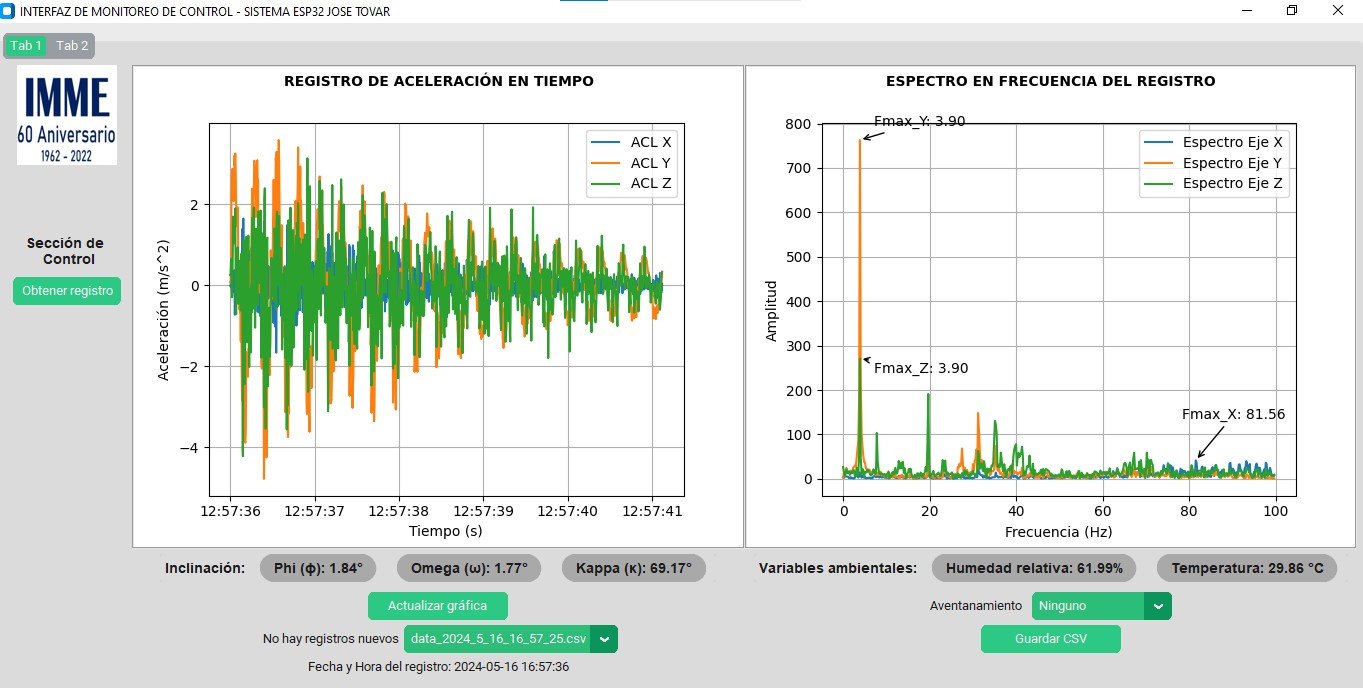
\includegraphics[width = \textwidth]{imagenes/cap3_resultados/Ensayos/VibLibreLastresSMARTSENSOR.jpg}
    \caption{Registro de vibración libre con lastres obtenido mediante el sensor inteligente.}
    \label{fig:libreGUI_CL}
\end{figure}

Al observar los resultados obtenidos en las figuras \ref{fig:libreGUI_CL} y \ref{fig:DAQlibreCL}, se pueden apreciar las similitudes entre los espectros en frecuencia de ambos sistemas, donde resaltan claramente la frecuencia de vibración que corresponde a la frecuencia en la dirección larga del sistema. En el caso del sensor inteligente, se obtuvo un valor de 3.90 Hz, mientras que en el sistema basado en la tarjeta PCI-6221 el valor es de 3.87 Hz, siendo el error entre ambos sistemas de apenas 0.03 Hz. Además de confirmarse que los datos obtenidos por el sensor inteligente son confiables y permiten caracterizar el comportamiento dinámico del sistema, se observa como el valor de esta frecuencia disminuyó respecto al valor de 4.6 Hz observado en las figuras \ref{fig:DAQlibreSL} y \ref{fig:libreGUI_SL}, demostrándose la capacidad del sistema de medir cambios en la respuesta natural del sistema producto de cambios en la masa del mismo.

%AMBIENTAL
\subsection{Vibración ambiental}

Este ensayo consistió en tomar registros de datos sin perturbar la estructura. Es decir, siendo esta excitada únicamente por factores naturales como el viento o el paso de personas.

En primer lugar, se observa en las figuras \ref{fig:DAQamb1} y \ref{fig:DAQamb2} la respuesta en tiempo y el espectro en frecuencia del sistema ante vibración ambiental.

\begin{figure}[H]
    \centering
    \subfloat[Aceleración en el tiempo del sistema ante vibración ambiental]{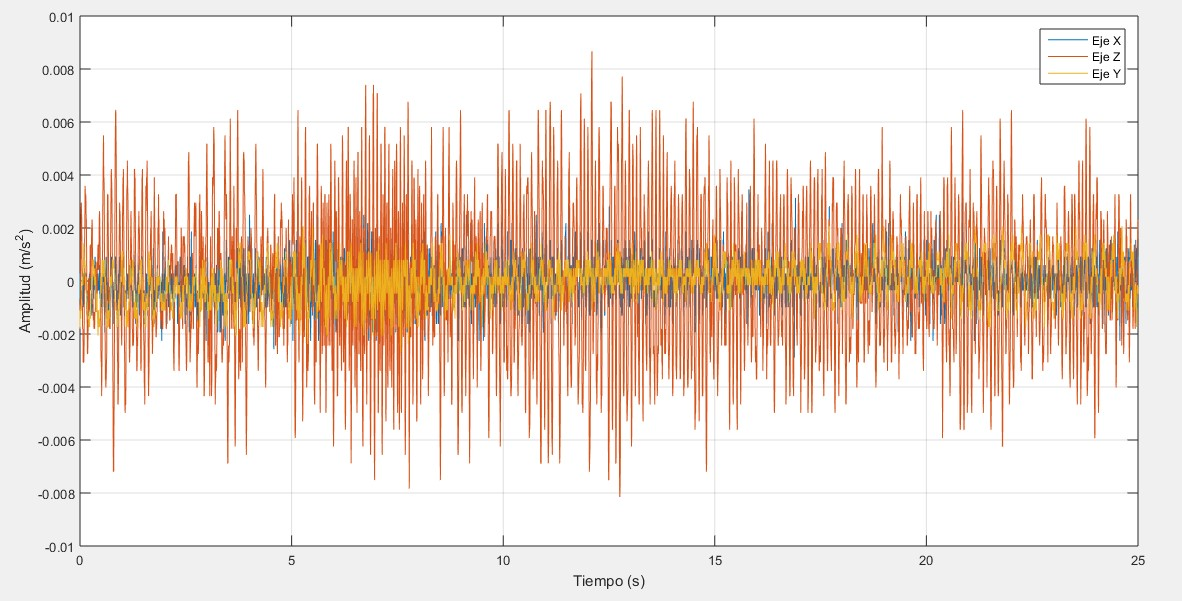
\includegraphics[width = \textwidth]{imagenes/cap3_resultados/Ensayos/AmplitudVibAmb2NIDAQ1.jpg}\label{fig:DAQamb1}}
    \hfill
    \subfloat[Espectro en frecuencia del sistema ante vibración ambiental]{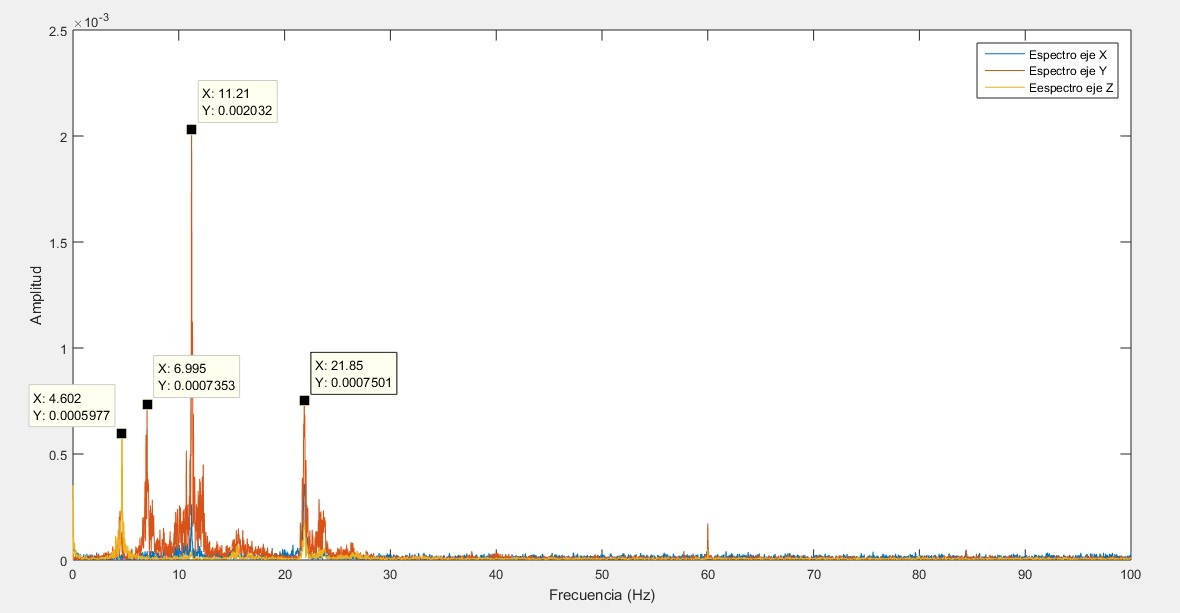
\includegraphics[width = \textwidth]{imagenes/cap3_resultados/Ensayos/VibAmb2EspectroNIDAQ1.jpg}\label{fig:DAQamb2}}
    \caption{Respuesta del sistema ante vibración ambiental según la tarjeta PCI-6221 de National Instruments}
    \label{fig:DAQAmb}
\end{figure}

En la figura \ref{fig:ambientalGUI} se observa la interfaz gráfica diseñada para el sensor inteligente al leer uno de los registros de vibración ambiental obtenido durante el ensayo:

\begin{figure}[H]
    \centering
    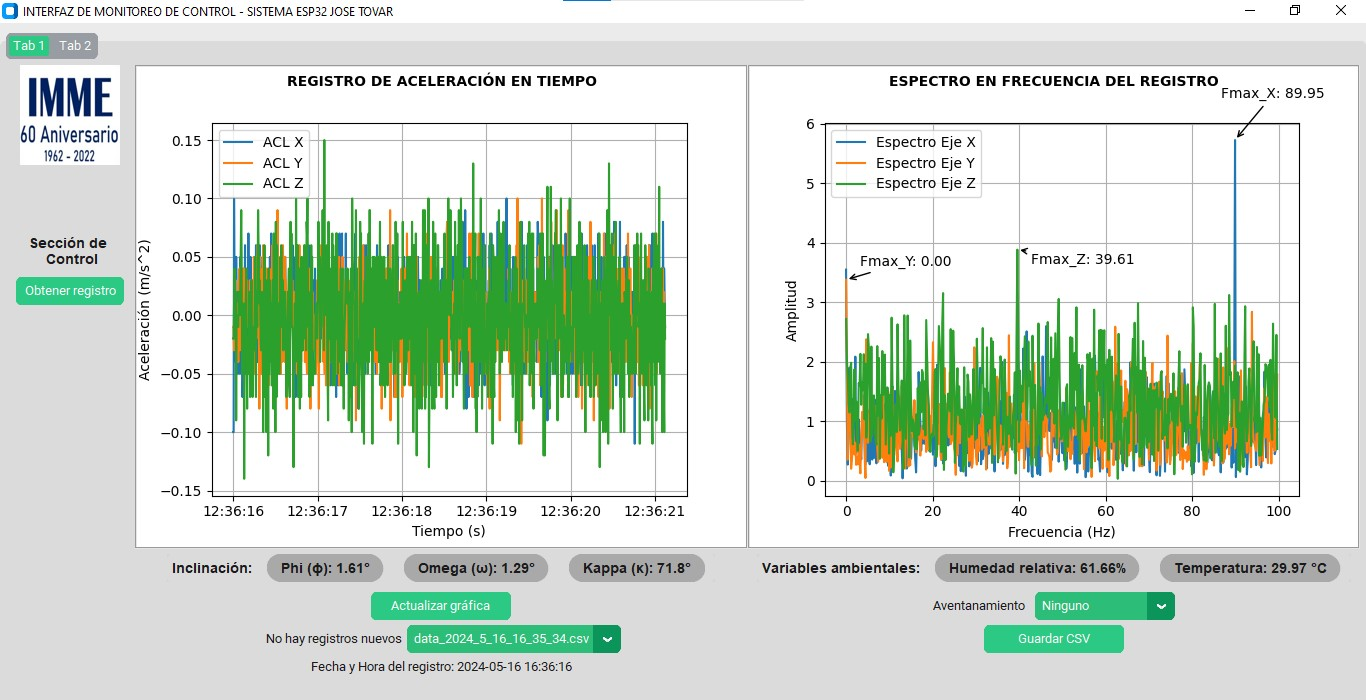
\includegraphics[width = \textwidth]{imagenes/cap3_resultados/Ensayos/VibAmb2SmartSensorGUI.jpg}
    \caption{Ventana de la interfaz gráfica diseñada con el registro de vibración ambiental obtenido.}
    \label{fig:ambientalGUI}
\end{figure}

Si bien los resultados obtenidos por vibración ambiental pueden verse por registro directamente en la interfaz, como se observa en la figura \ref{fig:ambientalGUI}, es conveniente concatenar varios archivos debido a la longitud de cada registro. Mientras mayor es el tamaño del registro, mayor resolución tendrá el espectro al tener más datos. Es decir, el $\Delta f$ mejora al aumentar la longitud de los registros.

Al concatenar registros es necesario aventanar cada registro, usando alguna función de aventanamiento como las definidas en la sección \ref{sec:aventanamiento}, para que evitar que se introduzcan al espectro cambios bruscos producto de la concatenación de archivos. En la figura \ref{fig:concatenados3} se observa el resultado de concatenar 3 registros de vibración ambiental que fueron tomados de forma sucesiva mientras se tomó el registro con la tarjeta PCI-6221 registrado en la figura \ref{fig:DAQamb1}. Para esto, se implementó un código en Python capaz de concatenar 3 archivos, generando un registro continuo utilizando la ventana de Hanning.

\begin{figure}[H]
    \centering
    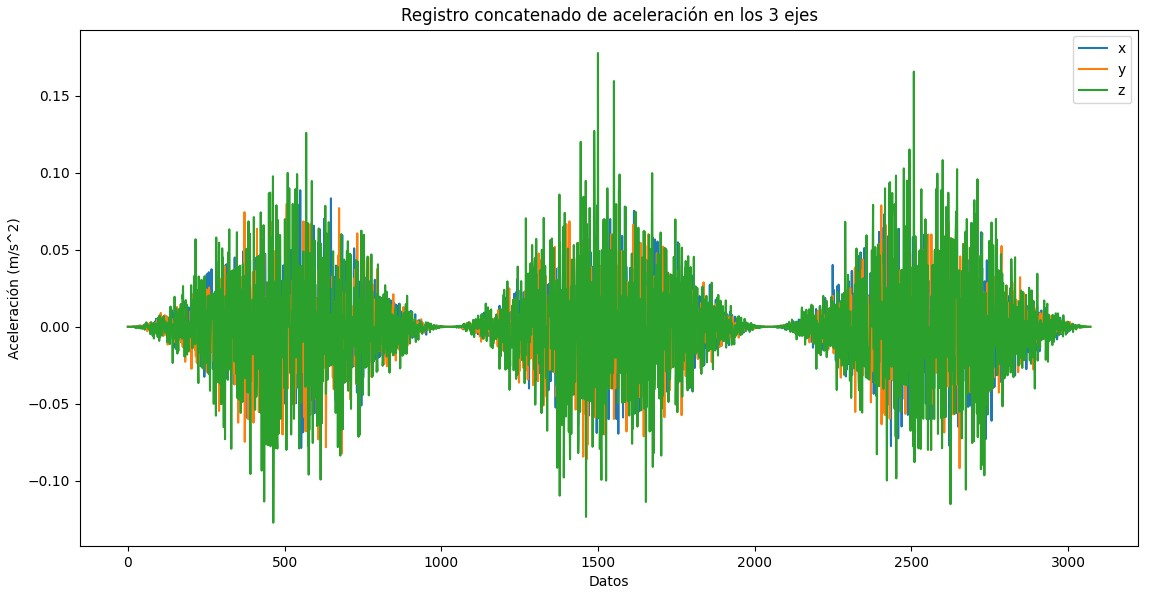
\includegraphics[width = \textwidth]{imagenes/cap3_resultados/Ensayos/AmplitudVibAmb2CONCATENADASMARTSENSOR.jpg}
    \caption{Forma del registro concatenado tras aventanamiento de Hanning utilizando Python.}
    \label{fig:concatenados3}
\end{figure}

Una vez concatenados, se procedió a ejecutar la FFT sobre los datos, obteniéndose el espectro de la figura \ref{fig:espectroconc}:

\begin{figure}[H]
    \centering
    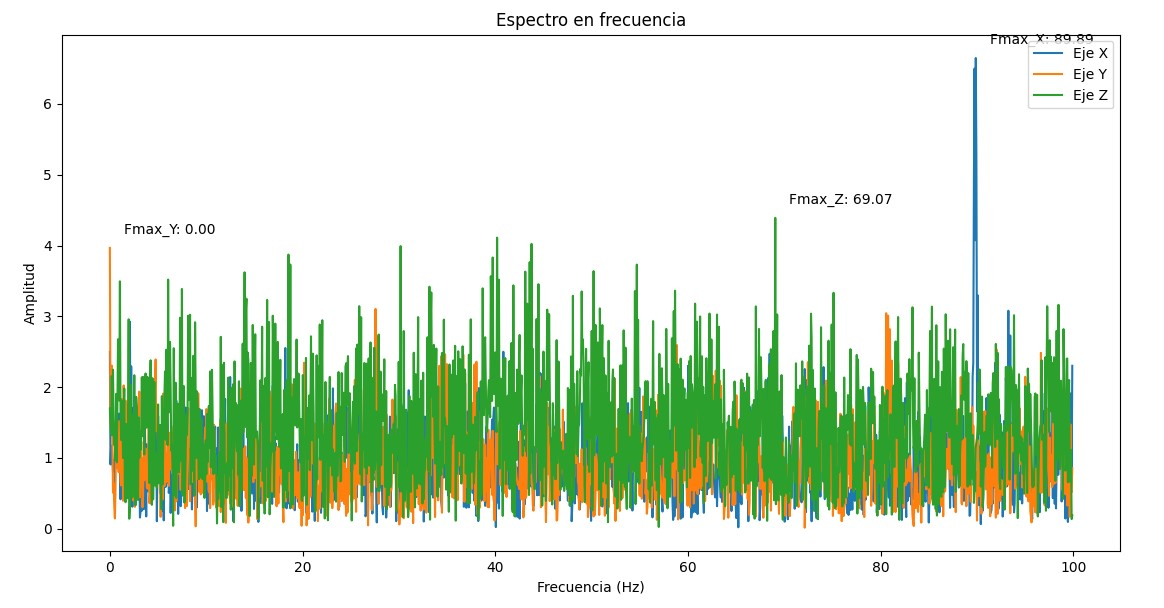
\includegraphics[width = \textwidth]{imagenes/cap3_resultados/Ensayos/VibAmb2EspectroCONC.jpg}
    \caption{Forma del espectro del registro concatenado.}
    \label{fig:espectroconc}
\end{figure}



Al comparar las figuras \ref{fig:espectroconc} y \ref{fig:DAQamb2} se observa que el espectro obtenido mediante el sensor inteligente no contiene los picos observados en el espectro obtenido por la tarjeta PCI-6221. Esto puede deberse al pobre acoplamiento entre el sensor inteligente y la estructura al estar este sobre una placa de prototipos, la cual a su vez se unió al sistema con yeso, evidenciándose en amplitudes bajas. Si bien el registro de la figura \ref{fig:ambientalGUI} muestra el comportamiento esperado por un registro de vibración ambiental en tiempo, para que el sensor sea capaz de captar los leves movimientos de la estructura en vibración ambiental, este debe estar acoplado al sistema, como es el caso de los acelerómetros Kinemetrics. A pesar de obtener estas discrepancias entre ambos espectros, el bajo nivel de ruido presentado por el sensor inteligente en vibraciones ambientales y la facilidad para concatenar registros debido al formato del mismo lo proyecta como un buen candidato para tomar registros de vibraciones ambientales siempre y cuando este se encuentre firmemente acoplado al sistema en estudio.
